\documentclass[a4paper,10pt]{article}
\usepackage[utf8x]{inputenc}
\usepackage{array}
\usepackage[pdftex]{graphicx}
\usepackage{hyperref}
\usepackage{listings}
\usepackage{enumitem}
\usepackage{color, colortbl}
\usepackage{longtable}
\usepackage{float}
\usepackage[compact]{titlesec}		% The 'compact' argument reduces spacing before/after headings

% Start ---- Fix for bug in issue 2.10.1 of titlesec package
\usepackage{etoolbox}

\makeatletter
\patchcmd{\ttlh@hang}{\parindent\z@}{\parindent\z@\leavevmode}{}{}
\patchcmd{\ttlh@hang}{\noindent}{}{}{}
\makeatother
% End ---- Fix for bug in issue 2.10.1 of titlesec package

\usepackage{verbatim}
\usepackage{fancyhdr}
\usepackage{parskip}
\usepackage{listings}

%---------------------------------------------
% Management of Captions
%---------------------------------------------
\usepackage[labelfont=bf]{caption}	% The caption label for tables and figures is bolded
\setlength{\abovecaptionskip}{0pt}	% Bring label close to figure or table
\renewcommand{\figurename}{Fig.}	% The caption label for figures is: "Fig."
\captionsetup[table]{singlelinecheck=off,justification=raggedright}	% Justify the table captions to the left

\pagestyle{fancy}

%---------------------------------------------
% Paragraph Layout
%---------------------------------------------
\setlength{\parindent}{0in}						% No indentation on first line of a new paragraph

%------------------------------------------------------------------------------------------
% Management of Headings
%------------------------------------------------------------------------------------------
% Define spacing to the left, before and after a subsection heading
%\titlespacing\subsubsection{8pt}{12pt plus 4pt minus 2pt}{-10pt plus 0pt minus 0pt}

% Introduce a page break before each section
\let\stdsection\section
\renewcommand\section{\newpage\stdsection}

%---------------------------------------------
% Headers and Footers
%---------------------------------------------
\renewcommand{\headrulewidth}{0.4pt}
\renewcommand{\footrulewidth}{0.4pt}

\lhead{PP-SP-COR-0001}
\chead{}
\rhead{Revision 1.2.2}
\lfoot{\textcopyright2012 P\&P Software GmbH. All Rights Reserved.} 
\cfoot{\vspace{5mm}
{\color{red}\verbatiminput{../commercial/LicensedTo.txt}}}
\rfoot{\thepage}

%---------------------------------------------
% Management of lists
%---------------------------------------------
\setlist{nolistsep}								% No extra vertical space around a list		
\newenvironment{fw_itemize}						% Control spacing between items in a list
{\begin{itemize}
  \setlength{\itemsep}{1mm}
  \setlength{\parskip}{0pt}
  \setlength{\parsep}{0pt}}
{\end{itemize}}

\newenvironment{fw_enumerate}					% Control spacing between items in an enumeration
{\begin{enumerate}
  \setlength{\itemsep}{1mm}
  \setlength{\parskip}{0pt}
  \setlength{\parsep}{0pt}}
{\end{enumerate}}

%---------------------------------------------
% Paragraph Layout
%---------------------------------------------
\setlength{\parindent}{0in}						% No indentation on first line of a new paragraph

%---------------------------------------------
% Define Environment for Requirement Tables without Notes
% Par #1: Requirement Title
% Par #2: Requirement Verification Method
% Par #3: Requirement Text
% Par #4: Requirement Justification
% Par #5: Requirement Implementation
% Par #6: Requirement Verification
%---------------------------------------------
\newenvironment{fw_req}[6]
{\addtocounter{subsubsection}{1}
	\hspace{0.2cm}\textbf{FW-\arabic{section}.\arabic{subsection}.\arabic{subsubsection}/#2
	\hspace{0.8cm} #1}
	\vspace{-10pt}
\begin{longtable}{p{2.7cm}P{8.5cm}}
\hline
\textsc{Requirement} & #3 \\
\textsc{Justification} & #4 \\
\textsc{Implementation} & #5  \\ 
\textsc{Verification} & #6  \\
\hline
}
{\end{longtable}}

%---------------------------------------------
% Define Environment for Requirement Tables with Notes
% Par #1: Requirement Title
% Par #2: Requirement Verification Method
% Par #3: Requirement Text
% Par #4: Requirement Notes
% Par #5: Requirement Justification
% Par #6: Requirement Implementation
% Par #7: Requirement Verification
%---------------------------------------------
\newenvironment{fw_req_note}[7]
{\addtocounter{subsubsection}{1}
	\hspace{0.2cm}\textbf{FW-\arabic{section}.\arabic{subsection}.\arabic{subsubsection}/#2
	\hspace{0.8cm} #1}
	\vspace{-10pt}
\begin{longtable}{p{2.7cm}P{8.5cm}}
\hline
\textsc{Requirement} & #3 \\
\textsc{Note} & #4 \\
\textsc{Justification} & #5 \\
\textsc{Implementation} & #6  \\ 
\textsc{Verification} & #7  \\
\hline
}
{\end{longtable}}
	
%---------------------------------------------
% Define table layout 
%---------------------------------------------
\renewcommand{\arraystretch}{1.5}	% add vertical padding

\newcolumntype{P}[1]{>{%			% define column with paragraphs
  \parskip=0.5\baselineskip%
  \advance\parskip by 0pt plus 2pt
  \setlength{\parfillskip}{30pt plus 1fil}}p{#1}}


%---------------------------------------------
% Definition of colours
%---------------------------------------------
\definecolor{dkgreen}{rgb}{0,0.6,0}
\definecolor{gray}{rgb}{0.5,0.5,0.5}
\definecolor{mauve}{rgb}{0.58,0,0.82}
\definecolor{lightblue}{RGB}{128,179,255}
\definecolor{lbcolor}{rgb}{0.9,0.9,0.9}
\definecolor{light-gray}{gray}{0.85}
 
%---------------------------------------------
% Options for the code listing boxes
%---------------------------------------------
\lstset{ 
  language=C,                % the language of the code
  aboveskip=\bigskipamount,			% vertical space above listing box
  basicstyle=\footnotesize\ttfamily,    % use small size and mono-space font
  numbers=left,                   % where to put the line-numbers
  numberstyle=\tiny\color{gray},  % the style that is used for the line-numbers
  stepnumber=1,                   % the step between two line-numbers. If it's 1, each line 
                                  % will be numbered
  numbersep=5pt,                  % how far the line-numbers are from the code
  backgroundcolor=\color{lbcolor},      % choose the background color. You must add \usepackage{color}
  showspaces=false,               % show spaces adding particular underscores
  showstringspaces=false,         % underline spaces within strings
  showtabs=false,                 % show tabs within strings adding particular underscores
  frame=single,                   % adds a frame around the code
  rulecolor=\color{black},        % if not set, the frame-color may be changed on line-breaks within not-black text (e.g. commens (green here))
  tabsize=2,                      % sets default tabsize to 2 spaces
  captionpos=b,                   % sets the caption-position to bottom
  breaklines=true,                % sets automatic line breaking
  breakatwhitespace=false,        % sets if automatic breaks should only happen at whitespace
  title=\lstname,                   % show the filename of files included with \lstinputlisting;
                                  % also try caption instead of title
  keywordstyle=\color{blue},          % keyword style
  commentstyle=\color{dkgreen},       % comment style
  stringstyle=\color{mauve},         % string literal style
  escapeinside={\%*}{*)},            % if you want to add a comment within your code
  morekeywords={*,...}               % if you want to add more keywords to the set
}
 
%---------------------------------------------
% Title Page
%---------------------------------------------
\title{\textsc{The Framework Profile} \\ \textsc{C1 Implementation} \\ \textsc{- USER REQUIREMENTS -}}
\date{13 October 2016}
\author{Alessandro Pasetti \& Vaclav Cechticky}


\begin{document}
\maketitle

\begin{center}
Revision 1.2.2 \\
PP-SP-COR-0001
\end{center}

\begin{center}
P\&P Software GmbH \\
High Tech Center 1 \\
8274 T\"{a}gerwilen \\
Switzerland \\
\vspace{2mm}
Web site: \url{www.pnp-software.com}\\
E-mail: \href{mailto:pnp-software@pnp-software.com}{\nolinkurl{pnp-software@pnp-software.com}} 
\end{center}


\begin{table}[ht]
\begin{center}
\begin{tabular}{p{11.7cm}}
\\
\hline
\end{tabular}
\end{center}
\end{table}
\begin{abstract}
This document defines, justifies, and verifies the User Requirements for the C1 Implementation of the FW Profile. The FW Profile is a specification-level modelling 
language defined as a restriction of UML. The core modelling constructs offered by the FW Profile are State Machines, Procedures (equivalent to UML's Activity Diagrams), and RT Containers (encapsulations of threads).
\par
The FW Profile is implementation-independent. The C1 Implementation is a C language implementation of the modelling concepts of the FW Profile. The main features of the C1 Implementation are: small memory footprint, small CPU demands, scalability, and
high reliability.
\par 
The C1 Implementation is provided with a Qualification Data Package which can be used to support the certification of applications built using its components.
\end{abstract}
\begin{table}[ht]
\begin{center}
\begin{tabular}{p{11.7cm}}
\\
\hline
\end{tabular}
\end{center}
\end{table}

%---------------------------------------------
% Table of contents and list of figures and requirements
%---------------------------------------------
\newpage
\tableofcontents

\newpage
\listoffigures
\listoftables
\lstlistoflistings

%---------------------------------------------
% Copyright notice
%---------------------------------------------

\newpage
\vspace*{\fill}
\begin{center}
No part of this publication may be reproduced, transmitted, transcribed, stored in any retrieval system, or translated into any language
by any means without express prior written permission of P\&P Software GmbH.
\end{center}

\begin{center}
Copyright \textcopyright 2012 P\&P Software GmbH. All Rights Reserved. 
\end{center}
\vspace*{\fill}

%---------------------------------------------
% Adjust distance between paragraphs (this cannot be done earlier or it also affects the TOC)
%---------------------------------------------
\setlength{\parskip}{3mm}						% Set distance between paragraphs

%---------------------------------------------
% Start of Document Text
%---------------------------------------------

\section{Change History}

This section lists the changes made in successive revisions of this document. Changes are classified according to their type. The change type is identified in the second column in the table according to the following convention:

\begin{itemize}[itemsep=0mm]
\item "\textbf{E}": Editorial or stylistic change
\item "\textbf{L}": Clarification of existing text
\item "\textbf{D}": A requirement or part of a requirement which was present in the previous revision has been deleted
\item "\textbf{C}": A requirement or part of a requirement which was presented in the previous revision has been changed
\item "\textbf{N}": A new requirement has been introduced
\end{itemize}

\begin{longtable}{|p{1.5cm}|p{1cm}|p{8cm}|}
\caption{Changes introduced in Revision 1.2.2} \\
\hline
\rowcolor{light-gray}
\textbf{Section} & \textbf{Type} & \textbf{Description} \\
\hline\hline
\endfirsthead
\rowcolor{light-gray}
\textbf{Section} & \textbf{Type} & \textbf{Description} \\
\hline\hline
\endhead
n.a. & E & Corrected reference number in \cite{ref:um}\\
\hline
\end{longtable}

\begin{longtable}{|p{1.5cm}|p{1cm}|p{8cm}|}
\caption{Changes introduced in Revision 1.2.1} \\
\hline
\rowcolor{light-gray}
\textbf{Section} & \textbf{Type} & \textbf{Description} \\
\hline\hline
\endfirsthead
\rowcolor{light-gray}
\textbf{Section} & \textbf{Type} & \textbf{Description} \\
\hline\hline
\endhead
n.a. & E & Corrected error in document reference number in page headers\\
\hline
\end{longtable}

\newpage

\begin{longtable}{|p{1.5cm}|p{1cm}|p{8cm}|}
\caption{Changes introduced in Revision 1.2.0} \\
\hline
\rowcolor{light-gray}
\textbf{Section} & \textbf{Type} & \textbf{Description} \\
\hline\hline
\endfirsthead
\rowcolor{light-gray}
\textbf{Section} & \textbf{Type} & \textbf{Description} \\
\hline\hline
\endhead
n.a. & L & Clarified formulation of abstract\\
\hline
n.a. & L & Added list of code listings to the table of contents\\
\hline
2 & L & Extended introduction to cover RT Containers \\
\hline
2.1 & E & Minor editorial corrections\\
\hline
3.3 & E & Minor editorial change in verification part of requirement FW-3.3.2; in requirement FW-3.3.3, corrected reference to: "\texttt{FwSmTestCaseCheck7}", to reference to: "\texttt{FwSmTestCaseCheck6}"; in requirement FW-3.3.5: corrected reference to section 5.2 to reference to section 4.2\\
\hline
3.3 & N & Added a note to requirement FW-3.3.2 to clarify the definition of "configuration" and modified requirement justification to reflect this definition \\
\hline
3.4 & E & In requirement FW-3.4.3: changed "\texttt{FwSmStart}" to "\texttt{FwSmStop}"\\
\hline
3.4 & E & Minor editorial change in implementation part of requirement FW-3.4.2 \\
\hline
3.5 & E & Minor editorial correction in justification part of requirement FW-3.5.2; in requirement FW-3.5.5: changed reference to section 5.2, to reference to section 4.2; fixed typo in verification part of requirement FW-3.5.6 \\
\hline
3.7 & E & Minor editorial change in justification part of requirement FW-3.7.5 \\
\hline
3.7 & C & Expanded the set of test case which verify requirement FW-3.7.5 \\
\hline
4.1 & C & Changed verification method of requirement FW-4.1.2 from 'A' to 'R' \\
\hline
4.3 & E & Fixed typos in requirement FW-4.3.1 \\
\hline
4.3 & N & Added a note to requirement FW-4.3.2 to clarify the definition of "configuration" and modified requirement justification to reflect this definition \\
\hline
4.4 & L & Fixed typos and improved formulation of requirement FW-4.4.2 \\
\hline
4.5 & L & Minor clarification in formulation of requirement FW-4.5.2 \\
\hline
5 & N & New section on functional requirements of RT Containers \\
\hline
6.1 & C & Changed verification method of requirement FW-6.1.1 from 'T' to 'R' \\
\hline
6.2 & C & Changed verification method of requirements in this section from 'T' to 'R' \\
\hline
6.2 & N & Added requirement FW-6.2.3 on RTD Internal Structure \\
\hline
6.2 & E & Minor editorial changes to requirements FW-6.2.1 and FW-6.2.2 \\
\hline
6.3 & C & Extended requirement FW-6.3.1 on code memory footprint to also cover RT container; changed verification method for all requirements in this section from "Testing" to "Review" \\
\hline
6.3 & N & Renumbered requirements FW-6.3.4 (State Machine Execution Time) and FW-6.3.5 (Procedure Execution Time) to, respectively, FW-6.3.5 and FW-6.3.6 and added a new requirement FW-6.3.4 cover memory footprint of RTDs \\
\hline
6.3 & E & Fixed typo in references to user manual \\
\hline
6.4 & C & Modified requirement FW-6.4.1 on concurrent environment to apply only to state machine and procedure parts of the C1 Implementation and changed its verification method from 'T' to 'R' \\
\hline
6.4 & N & Added requirement FW-6.4.2 to cover concurrent use of RT containers \\
\hline
6.5 & C & Modified formulation of requirement FW-6.5.1 on Test Coverage to refer to "system calls" rather than just "calls to \texttt{malloc} function"\\
\hline
6.5 & N & New requirement FW-6.5.2 on stress testing of RT containers \\
\hline
6.6 & C & Restricted requirement FW-6.6.1 on external libraries to state machine and procedure part of the C1 Implementation; changed verification method for this requirement  from 'T' to 'R' \\
\hline
6.6 & N & Added new requirement FW-6.6.2 on use of POSIX-compliant library \\
\hline
6.6 & E & Removed erroenous reference to appendix E from requirement FW-6.6.1 \\
\hline
A & N & Added section A.3 on implementation of RT Container Concept \\
\hline
A.2 & E & Fixed typo in introductory text of this section \\
\hline
B & E & In table 7: fixed typo in test case for \texttt{smNullCState} and in description of \texttt{smUndefinedTransSrc}; in table 8: changed \texttt{smUnreachablePNode} to \texttt{smUnreachableDNode}; in table 9: changed \texttt{FwSmTestCaseCheck4} to \texttt{FwPrTestCaseCheck4} and deleted entry for \texttt{FwSmTestCaseTransErr2} from bottom row of table \\
\hline
B & D & Deleted \texttt{FwPrTestCaseCheck3} from verification of \texttt{prTooManyActions}; deleted \texttt{FwPrTestCaseCheck7} from verification of \texttt{prIllNOfOutFlows} \\
\hline
C & N & Added section C.3 on verification Start/Stop behaviour of RT Containers \\
\hline
C.2 & E & Fixed typos in introductory text of this section and in first column of table 12\\
\hline
D.1 & E & Deleted duplicated entry for \texttt{FwSmTestCaseExecute3} from table 14 \\
\hline
D.1 & D & Deleted entry for \texttt{FwSmTestTrans3} from table 15 \\
\hline
D.2 & D & Deleted entry for \texttt{FwPrTestCaseExecute5} from first line of table 16 \\
\hline
E & N & New appendix section on verification of notification behaviour of RT Containers\\
\hline
\end{longtable}

\newpage

\begin{longtable}{|p{1.5cm}|p{1cm}|p{8cm}|}
\caption{Changes introduced in Revision 1.1.0} \\
\hline
\rowcolor{light-gray}
\textbf{Section} & \textbf{Type} & \textbf{Description} \\
\hline\hline
\endfirsthead
\rowcolor{light-gray}
\textbf{Section} & \textbf{Type} & \textbf{Description} \\
\hline\hline
\endhead
3.2 & L & Replaced reference to Acceptance Test Procedure document with reference to User Manual in verification part of requirement FW-3.2.2 \\
\hline
3.5 & E & Fixed typo in requirement FW-3.5.2 \\
\hline
3.5 & N & Added new requirement FW-3.5.3 on the order of evaluation of guards \\
\hline
3.7 & L & Replaced reference to Acceptance Test Procedure document with reference to User Manual in verification part of requirement FW-3.7.3 \\
\hline
4.2 & L & Replaced reference to Acceptance Test Procedure document with reference to User Manual in verification part of requirement FW-4.2.3 \\
\hline
4.5 & N & Added new requirement FW-4.5.3 on the order of evaluation of guards \\
\hline
4.7 & L & Replaced reference to Acceptance Test Procedure document with reference to User Manual in verification part of requirement FW-4.7.3 \\
\hline
6.1 & L & Replaced reference to Acceptance Test Procedure document with reference to User Manual in verification part of requirement FW-6.1.2 \\
\hline
6.5 & L & Replaced reference to Acceptance Test Procedure document with reference to User Manual in verification part of requirement FW-6.5.1 \\
\hline
B & N & Added test cases to verify presence of unreachable states and unreachable pseudo-states in a SMD; Added test cases to verify presence of unreachable nodes in a PRD \\
\hline
\end{longtable}

\newpage


\section{Introduction}
This document defines, justifies and verifies the user requirements for the \emph{C1 Implementation}. The C1 Implementation is a C-language implementation of the State Machine Concept, of the Procedure Concept, and of the RT Container Concept of the \emph{Framework (FW) Profile}. The FW Profile is a specification-level modelling language defined as a restriction of UML. The state machine concept of the FW Profile is modelled on the state machine concept of UML and the procedure concept of the FW Profile is modelled on the activity diagram concept of UML. The RT container concept is specific to the FW Profile. The FW Profile is defined in \cite{ref:fwprofile}. 

\subsection{Intended Use of C1 Implementation}\label{sec:intendedUse}
Although the C1 Implementation can be used wherever there is a need to implement a state machine or procedure concept or a threading model with a clear semantics, the high reliability of the implementation, the emphasis placed on formally specifying and verifying its expected behaviour, and the small demands on memory and processing resources mean that the C1 Implementation is especially well-suited for mission-critical embedded applications. 

Thus, the intended use of the C1 Implementation is to support the implementation of the state machine, procedure, and RT container concepts of the FW Profile for mission-critical embedded applications.

\subsection{Requirement Definition}\label{sec:reqDef}
Requirements are defined in tables with the following format:

\hspace{0.2cm}\textbf{FW-'x'/'V' \hspace{0.9cm} $\langle$Requirement Title$\rangle$}
\vspace{-10pt}

\begin{longtable}{p{2.7cm}P{8.5cm}}
\hline
\textsc{Requirement} & $\langle$Formulation of requirement$\rangle$ \\
%\hline
\textsc{Note} & $\langle$Explicatory notes for requirement$\rangle$ \\
%\hline
\textsc{Justification} & $\langle$Justification of requirement$\rangle$ \\
%\hline
\textsc{Implementation} & $\langle$Dscription of how requirement is implemented$\rangle$ \\ 
%\hline
\textsc{Verification} & $\langle$Dscription of how requirement is verified$\rangle$ \\
\hline
\end{longtable}

Here, the suffix 'x' is a numerical identifier which uniquely identifies the requirement
within this document. The suffix 'V' identifies the verification method for the requirement according to the convention presented in section \ref{sec:reqVer}.

The explicatory notes are appended to the definition of the requirements where there is a need to clarify the terms which are used in their formulation.

In addition to their definition, this document also provides the following information for each requirement: a justification of the requirement; a description of how the requirement is implemented; and a description of how the requirement is verified. 

\subsubsection{Requirement Justification}
For each requirement, a \emph{justification} is provided which \emph{validates} the requirement. Requirements are justified with respect to the intended use of the C1 Implementation. The intended use of the C1 Implementation is to support the implementation of the State Machine, Procedure and RT Container concepts of the FW Profile for mission-critical embedded applications (see section \ref{sec:intendedUse}).  Hence, a requirement is justified in proportion to its ability to further the adequacy of the C1 Implementation to support the implementation of the FW Profile in an environment where memory and processing resources are constrained and where reliability is of paramount importance. 

\subsubsection{Requirement Implementation}
For each requirement, the function or data structure or other code-level construct in the source code which implements it is identified.

\subsubsection{Requirement Verification}\label{sec:reqVer}
Verification information is provided for each requirement to demonstrate the correct implementation of the requirement. The following verification methods are possible:

\begin{fw_itemize}
\item Verification by Review ('R'): the requirement is verified by inspecting the code or its documentation.
\item Verification by Analysis ('A'): the requirement is verified by analysing the code, possibly with the help of a tool.
\item Verification by Test ('T'): the requirement is verified by one or more test cases in the Test Suite.
\end{fw_itemize}

One single verification method is defined for each requirement. 
This is identified as part of the requirement definition (see the description of the requirement format in section \ref{sec:reqDef}).

The Test Suite which is used for the verification by test is a complete application which demonstrates all aspects 
of the behaviour of the state machine, procedure, and RT container implementation. 
It consists of a sequence of Test Cases which are independent of each other. 
Each Test Case focuses on one particular functional aspect of the C1 Implementation. 
The Test Suite is distributed with the C1 Implementation.
It is documented as part of the Doxygen documentation for the C1 Implementation and is described in the C1 Implementation User Manual (see reference \cite{ref:um}).


%=============================================================================
% Introduce a page break before each sub-section
\let\stdsubsection\subsection
\renewcommand\subsection{\newpage\stdsubsection}
%=============================================================================


%=============================================================================
\section{State Machine - Functional Requirements}\label{sec:smFncReqs}
This section defines the functional requirements for the State Machine part of the C1 Implementation. 
The functional requirements are those which define the functional behaviour of the state machines in the C1 Implementation.

%=============================================================================
%\subsection{Implementation of State Machine Concept}\label{req:implFwProfileSM}

%------------{Implementation of State Machine Concept}
\begin{fw_req}{Implementation of State Machine Concept}{R}
{The C1 Implementation shall implement the state machine concept of the FW Profile of \cite{ref:fwprofile}.}
%-----------------------------------------------------------------------------
{The intended use of the C1 Implementation is to support the implementation of the state machine concept of the FW Profile.}
%-----------------------------------------------------------------------------
{The state machine behaviour specified by the FW Profile is implemented 
by the \texttt{FwSmCore.h} interface of the C1 Implementation.} 
%-----------------------------------------------------------------------------
{The FW Profile defines state machines in terms of their \emph{elements} 
and of their \emph{behaviour}. 
The state machine behaviour is in turn defined in terms of three operations which can be performed 
upon a state machine (\textit{start}, \textit{stop}, and \textit{command transition}).
Appendix \ref{Appendix_A_Implementation_SM_Concept} shows how each state machine element is 
mapped to a data structure in the C1 Implementation and how each state machine operation is 
mapped to a function in the \texttt{FwSmCore.h} interface of the C1 Implementation.}
\end{fw_req}

%=============================================================================
\subsection{State Machine Descriptor (SMD) Requirements}\label{req:SMD}

%------------{State Machine Descriptor (SMD)}
\begin{fw_req}{State Machine Descriptor (SMD)}{R}
{It shall be possible to address and to manipulate a state machine 
as a single entity (the \emph{State Machine Descriptor} or SMD).}
%-----------------------------------------------------------------------------
{The intended use of the C1 Implementation is to provide modules 
which can be deployed within another application. 
The definition of the SMD simplifies the interface between the modules of the C1 Implementation 
and the user application.}
%-----------------------------------------------------------------------------
{The SMD is manipulated as an instance of type \texttt{FwSmDesc\_t}.} 
%-----------------------------------------------------------------------------
{A state machine is represented by an instance of type 
\texttt{struct FwSmDesc} and is manipulated as an instance of type 
\texttt{FwSmDesc\_t} (a pointer to \texttt{struct FwSmDesc}).
All functions which operate on a state machine take an instance of this type as their argument.}
\end{fw_req}

%------------{SMD Encapsulation}
\begin{fw_req}{SMD Encapsulation}{R}
{The SMD shall encapsulate all the information defining the configuration and the current state of its state machine.}
%-----------------------------------------------------------------------------
{The intended use of the C1 Implementation is to provide modules which can be deployed within another application. 
The encapsulation of all information related to a state machine in a single data structure simplifies the interface between the modules of the 
C1 Implementation and the user application.}
%-----------------------------------------------------------------------------
{The SMD is defined as an instance of type \texttt{struct FwSmDesc}.} 
%-----------------------------------------------------------------------------
{The SMD models all the elements of a state machine (see 
section \ref{Appendix_A_Implementation_SM_Concept}) which define its configuration.
It models the current state of a state machine in field \texttt{curState}.}
\end{fw_req}

%=============================================================================
\subsection{Creation Requirements}\label{req:creationInterface}
%=============================================================================

%------------{Creation Interface}
\begin{fw_req}{Creation Interface}{T}
{ The C1 Implementation shall provide an interface through which a new SMD can be created.}
%-----------------------------------------------------------------------------
{Applications which wish to manipulate a state machine must first create the SMD which represents it.}
%-----------------------------------------------------------------------------
{The state machine creation interface is implemented in \texttt{FwSmDCreate.h} and \texttt{FwSmSCreate.h}.} 
%-----------------------------------------------------------------------------
{In the test suite, test state machines are used. The test state machines are created in functions with names like: \texttt{FwSmMakeTest<SM\_Name>}. 
These make functions exercise all SMD creation functions offered by the C1 Implementation.}
\end{fw_req}


%------------{Dynamic and Static Creation}
\begin{fw_req_note}{Dynamic and Static Creation}{T}
{ It shall be possible to create a new SMD either statically or dynamically.}
{The term \emph{static} refers to an instantiation process which does not rely on dynamic memory
allocation.}
%-----------------------------------------------------------------------------
{Dynamic creation of state machine is convenient but may be forbidden in mission-critical applications.}
%-----------------------------------------------------------------------------
{Dynamic state machine creation is implemented in \texttt{FwSmDCreate.h}. Static state machine 
creation is implemented in \texttt{FwSmSCreate.h}.} 
%-----------------------------------------------------------------------------
{In the test suite, test state machines are used. By default, the test state machines are created dynamically in functions with names like: \texttt{FwSmMakeTest<SM\_Name>}. 
Static creation of state machines is demonstrated in make functions with names like: \texttt{FwSmMakeTest<SM\_Name>Static}.}
\end{fw_req_note}


%------------{Release of SMD}
\begin{fw_req}{Release of SMD}{T}
%----------------------------------------------------------------------------
{If an SMD is created dynamically, then it shall also be possible to destroy it dynamically by releasing the memory 
that was allocated to it.}
%-----------------------------------------------------------------------------
{The target applications for the C1 Implementation are mission-critical applications. In this domain, dynamic 
memory allocation is only allowed if the means are available to reclaim the dynamically allocated memory.}
%-----------------------------------------------------------------------------
{Functions \texttt{FwSmRelease} and \texttt{FwSmReleaseRec} are provided in \texttt{FwSmDCreate.h} to release 
the memory allocated when a new SMD is created dynamically.} 
%-----------------------------------------------------------------------------
{In most Test Cases in the  Test Suite application, SMDs are created dynamically and the memory they use is then released before the end of the test. 
In the Acceptance Test for the C1 Implementation (see \cite{ref:um}), the Test Suite is run 
with the Valgrind tool and it is verified that no memory leaks occur and 
that all memory allocated dynamically is then released in an orderly way.}
%-----------------------------------------------------------------------------
\end{fw_req}


%======================================================================================
\subsection{Configuration Requirements}\label{req:configInterface}
%======================================================================================

%------------{Configuration Interface}
\begin{fw_req}{Configuration Interface}{T}
%----------------------------------------------------------------------------
{The C1 Implementation shall provide an interface through which an SMD can be configured and made to match 
the characteristics of a certain state machine.}
%-----------------------------------------------------------------------------
{Applications which wish to manipulate a state machine must configure it before they can send transition commands to it.}
%-----------------------------------------------------------------------------
{The state machine configuration interface is implemented in \texttt{FwSmConfig.h}.} 
%-----------------------------------------------------------------------------
{In the test suite, test state machines are configured. The Test Suite exercises all configuration 
functions in \texttt{FwSmConfig.h}.}
%----------------------------------------------------------------------------
\end{fw_req}


%------------{Reconfiguration of an SMD}
\begin{fw_req_note}{Reconfiguration of an SMD}{T}
%----------------------------------------------------------------------------
{It shall not be possible to re-configure an SMD which has already been configured.}
%-----------------------------------------------------------------------------
{The term configuration refers to the operations which must be performed on a newly-created SMD before it can be started.}
%-----------------------------------------------------------------------------
{ The C1 Implementation targets mission-critical applications. 
In this domain, dynamic reconfiguration of state machines would be regarded as unsafe 
because it makes it harder to determine behaviour through static analysis.}
%-----------------------------------------------------------------------------
{ The size of a state machine (the number of states, of choice pseudo-states, of transitions, of actions, and of guards) can only be set when its SMD is created and cannot therefore be changed after creation. 

After creation, three configuration operations must be performed on an SMD: (a) definition of taddhe states specified when the SMD was created (with function \texttt{FwSmAddState}); 
(b) definition of the choice pseudo-states specified when the SMD was created (with function \texttt{FwSmAddChoicePseudoState}); 
(c) definition of the transitions specified when the SMD was created (with functions with names like: \texttt{FwSmAddTrans*}). 
All of these operations add an item to an SMD (either a state, or a choice pseudo-state, 
or a transition). 
The SMD uses data structures with a fixed size. The configuration operations 
check whether there is space for the new item. 
If this is not the case, they return with an error. Since no functions are available 
for \emph{removing} items from an SMD, it follows that, once an SMD has been configured, 
any attempt to execute a configuration function will fail with an error.} 
%-----------------------------------------------------------------------------
{Test Case \texttt{FwSmTestCaseConfigErr2} verifies that attempts to 
reconfigure a state machine which has already been configured result in errors. 
More specifically, the test case creates and configures a state machine and then verifies 
that the following operations fail: (a) adding a new state; (b) re-defining an existing state; 
(c) adding a new choice pseudo-state; (d) re-defining an existing choice pseudo-state; 
(e) adding a new transition; (f) re-defining an existing transition.}
%----------------------------------------------------------------------------
\end{fw_req_note}


%------------{Configuration Check}
\begin{fw_req}{Configuration Check}{T}
%----------------------------------------------------------------------------
{It shall be possible to check the completeness and correctness of the configuration of an SMD (\emph{Configuration Check}).}
%-----------------------------------------------------------------------------
{The C1 Implementation targets mission-critical applications. 
In this domain, it is important to be able to periodically check the integrity of an application.}
%-----------------------------------------------------------------------------
{The Configuration Check is implemented in functions 
\texttt{FwSmCheck} and \texttt{FwSmCheckRec}. These functions verify 
the completeness of the state machine configuration by checking that all states, 
choice pseudo-states, and transitions of a state machine have been 
defined. The correctness of the configuration of the state machine is checked indirectly 
as follows. 
The configuration functions in \texttt{FwSmConfig.h} perform a correctness check before 
executing a configuration request. If a violation of correctness is detected, it is reported 
by setting the \emph{error code} field of the SMD. 
The Configuration Check verifies that the error code is set to "success". 
This value implies that no configuration errors have been detected and that therefore 
the configuration of the SMD is correct.} 
%-----------------------------------------------------------------------------
{The ability of the Configuration Check to report an incomplete 
configuration is verified in the test cases: \texttt{FwSmTestCaseCheck1} 
to \texttt{FwSmTestCaseCheck6}. The test cases which verify the ability of the 
Configuration Check to detect incorrect configuration requests are identified 
in Appendix \ref{Appendix_B_Error_Checks}.}
%----------------------------------------------------------------------------
\end{fw_req}


%------------{Configuration Status Print}
\begin{fw_req}{Configuration Status Print}{T}
%----------------------------------------------------------------------------
{It shall be possible to extract and print the configuration 
information of an SMD.}
%-----------------------------------------------------------------------------
{This capability is useful during debugging.}
%-----------------------------------------------------------------------------
{The configuration print service is implemented in function 
\texttt{FwSmPrintConfig}.} 
%-----------------------------------------------------------------------------
{The configuration print service is verified in test cases 
\texttt{FwSmTestCasePrint1} and \texttt{FwSmTestCasePrint2}.}
%----------------------------------------------------------------------------
\end{fw_req}


%------------{Configuration Constraints}
\begin{fw_req}{Configuration Constraints}{R}
%----------------------------------------------------------------------------
{The SMD configuration interface shall enforce the syntactical 
constraints C1 to C8 defined in section 4.2 of 
the FW Profile Definition in \cite{ref:fwprofile}.}
%-----------------------------------------------------------------------------
{The C1 Implementation is intended to support the state machine 
concept of the FW Profile. Enforcement of these 
constraints is part of the support of the FW Profile model of a  state machine.}
%-----------------------------------------------------------------------------
{ Enforcement of the constraints is achieved by the way 
the \texttt{FwSmAddTrans*} functions in 
\texttt{FwSmConfig.h} are defined: their interfaces make definition of a transition 
which violates a constraint impossible.} 
%-----------------------------------------------------------------------------
{\textbf{Constraint C1} ("The same pseudo-state cannot be both source and target for
 a transition") is enforced because the only 
\texttt{FwSmAddTrans*} functions which allow definition of a transition between two 
pseudo-states are \texttt{FwSmAddTransIpsToCps} 
and \texttt{FwSmAddTransCpsToFps} and these functions guarantee that source and destination 
are different.
\par
\textbf{Constraint C2} ("The source and target of a transition cannot both be choice 
pseudo-states") is enforced because there is no 
\texttt{FwSmAddTrans*} function which allows definition of a transition with a choice 
pseudo-state at both ends.
\par
\textbf{Constraint C3} ("The transition that has the initial pseudo-state as source 
can have neither a guard nor a trigger") is enforced 
because the transition out of the initial pseudo-state is defined through functions 
\texttt{FwSmAddTransIps*} and these functions allow neither a guard nor a trigger to be defined.
\par
\textbf{Constraint C4} has been deleted.
\par
\textbf{Constraint C5} ("Transitions that have a choice pseudo-state as source cannot have 
a transition trigger") is enforced because the 
transitions out of a choice pseudo-state are defined through functions 
\texttt{FwSmAddTransCps*} and these functions do not allow a trigger 
to be attached to the transition.
\par 
\textbf{Constraint C6} has been deleted.
\par
\textbf{Constraint C7} ("Transitions that have a state as a source must have a 
transition command") is enforced because the transitions out of 
a state are defined through functions \texttt{FwSmAddTransSta*} and these functions 
require definition of a transition command.
\par 
\textbf{Constraint C8} ("Transitions can only link states and/or pseudo-states that 
belong to the same state machine") is enforced because no 
functions are provided to let states or pseudo-states of different state machines be 
linked together through a transition.}
%----------------------------------------------------------------------------
\end{fw_req}

%======================================================================================
\subsection{Start and Stop Requirements}\label{req:startStopInterface}
%======================================================================================

%------------{Start and Stop Interface}
\begin{fw_req}{Start and Stop Interface}{T}
%----------------------------------------------------------------------------
{ The C1 Implementation shall provide an interface through 
which the state machine represented by an SMD can be started, 
stopped and queried for its present Started/Stopped status.}
%-----------------------------------------------------------------------------
{The Start/Stop operations are defined by the FW Profile. 
The intended use of the C1 Implementation is to support 
the implementation of the state machine concept of the FW Profile.}
%-----------------------------------------------------------------------------
{The Start/Stop operations are implemented in \texttt{FwSmCore.h}
 by functions \texttt{FwSmStart} and \texttt{FwSmStop}. 
The status query operation is implemented by function \texttt{FwSmIsStarted}.} 
%-----------------------------------------------------------------------------
{The Test Cases in the Test Suite start, stop and query state machines 
through the functions of \texttt{FwSmCore.h} and this interface has 100\% coverage of its implementation.}
%----------------------------------------------------------------------------
\end{fw_req}


%------------{Start Behaviour}
\begin{fw_req}{Start Behaviour}{T}
%----------------------------------------------------------------------------
{The Start interface shall implement the behaviour defined in the activity diagram on the left-hand side of 
Figure \ref{fig:SmStartStop}.}
%-----------------------------------------------------------------------------
{The activity diagram of Figure \ref{fig:SmStartStop} is the same as in the FW Profile definition of \cite{ref:fwprofile}.}
%-----------------------------------------------------------------------------
{The Start interface is implemented in function \texttt{FwSmStart}.} 
%-----------------------------------------------------------------------------
{The verification of this requirement is done in Appendix
\ref{Appendix_C_SM_Start_Stop} where it is shown that all branches of the activity diagrams of
\ref{fig:SmStartStop} are covered by at least one Test Case in the Test Suite.}
%----------------------------------------------------------------------------
\end{fw_req}


%------------{Stop Behaviour}
\begin{fw_req}{Stop Behaviour}{T}
%----------------------------------------------------------------------------
{The Stop interface shall implement the behaviour defined in 
the activity diagram on the right-hand side of Figure \ref{fig:SmStartStop}.}
%-----------------------------------------------------------------------------
{The activity diagram of Figure \ref{fig:SmStartStop} is the 
same as in the FW Profile Definition Document of \cite{ref:fwprofile}.}
%-----------------------------------------------------------------------------
{The Stop interface is implemented in the function \texttt{FwSmStop}.} 
%-----------------------------------------------------------------------------
{The verification of this requirement is done in Appendix \ref{Appendix_C_SM_Start_Stop} where it is shown that all branches of the activity diagrams of \ref{fig:SmStartStop} are covered by at least one Test Case in the Test Suite.}
%----------------------------------------------------------------------------
\end{fw_req}


%======================================================================================
\begin{figure}[h]
 \centering
 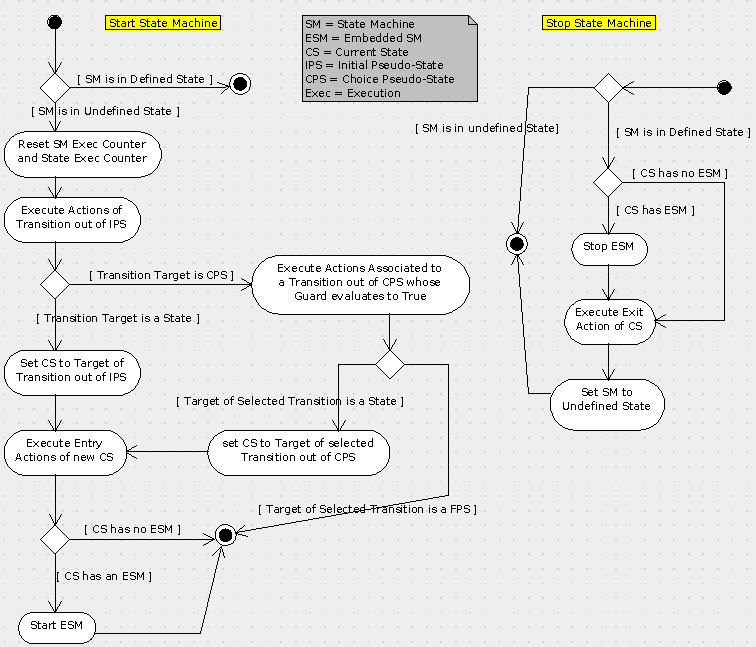
\includegraphics[scale=0.415,keepaspectratio=true]{../images/SM_StartStop.png}
 \caption{State Machine Start/Stop Behaviour}
 \label{fig:SmStartStop}
\end{figure}
%======================================================================================


%======================================================================================
\subsection{Transition Command Requirements}\label{req:transCmdInterface}
%======================================================================================

%------------{Transition Command Interface}
\begin{fw_req_note}{Transition Command Interface}{T}
%----------------------------------------------------------------------------
{The C1 Implementation shall provide an interface through which 
Transition Commands can be sent to a state machine.}
%-----------------------------------------------------------------------------
{A Transition Command is a command sent to a State Machine requesting it 
to perform a certain state transition.}
%-----------------------------------------------------------------------------
{The commanding of a state machine through transition commands 
is defined by the FW Profile. 
The intended use of the C1 Implementation is to support the implementation of the state
 machine concept of the FW Profile.}
%-----------------------------------------------------------------------------
{The Transition Command operations are implemented in 
\texttt{FwSmCore.h} by functions \texttt{FwSmMakeTrans} and \texttt{FwSmExecute}.} 
%-----------------------------------------------------------------------------
{The Test Cases in the Test Suite send transition commands 
to state machines through the functions of \texttt{FwSmCore.h} and this interface 
has 100\% coverage of its implementation.}
%----------------------------------------------------------------------------
\end{fw_req_note}


%------------{Transition Command Behaviour}
\begin{fw_req}{Transition Command Behaviour}{T}
%----------------------------------------------------------------------------
{The C1 Implementation shall implement the Transition Command behaviour defined in the activity diagrams of Figures \ref{fig:SmTransCmd} and \ref{fig:SmExecutingTransCmd}.}
%-----------------------------------------------------------------------------
{The activity diagrams of Figures \ref{fig:SmTransCmd} and \ref{fig:SmExecutingTransCmd} are the same as the activity diagrams in reference \cite{ref:fwprofile} which define the handling of transition commands in the FW Profile.}
%-----------------------------------------------------------------------------
{The Transition Command behaviour is implemented in functions \texttt{FwSmMakeTrans} and (only for the "Execute" Transition Command) \texttt{FwSmExecute}.} 
%-----------------------------------------------------------------------------
{The verification of this requirement is done in Appendix \ref{Appendix_D_SM_Trans} where it is shown that every branch of the activity diagrams of Figures \ref{fig:SmTransCmd} and \ref{fig:SmExecutingTransCmd} is covered by at least one Test Case in the Test Suite.}
%----------------------------------------------------------------------------
\end{fw_req}


%======================================================================================
\begin{figure}
 \centering
 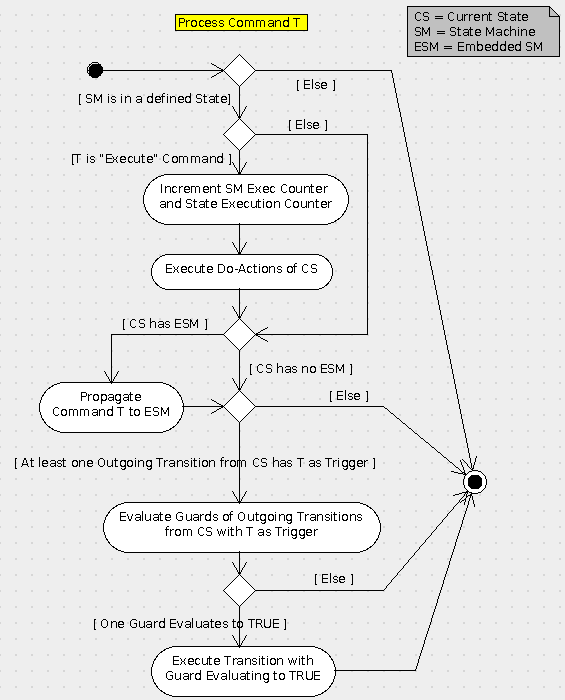
\includegraphics[scale=0.55,keepaspectratio=true]{../images/SM_CmdProcessing.png}
 \caption{Logic for Processing Transition Commands by a State Machine}
 \label{fig:SmTransCmd}
\end{figure}
%======================================================================================

%======================================================================================
\begin{figure}[h]
 \centering
 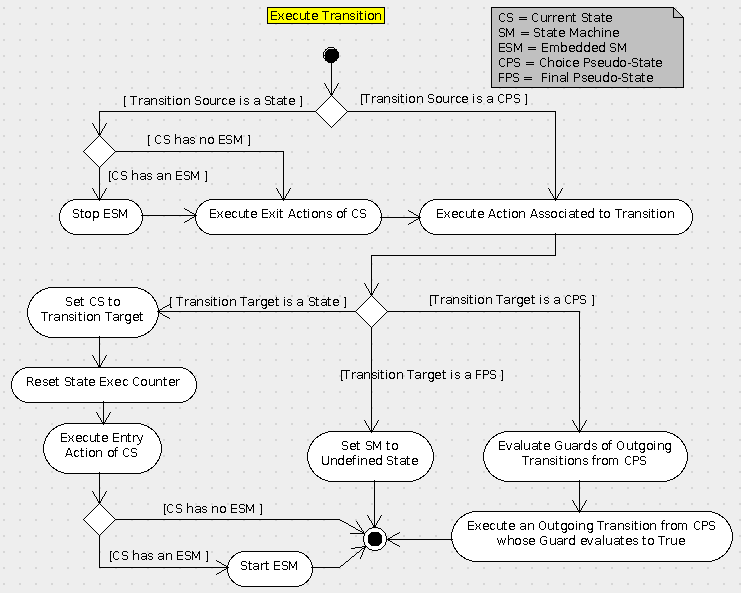
\includegraphics[scale=0.465,keepaspectratio=true]{../images/SM_TransitionExecution.png}
 \caption{Logic for Executing Transitions in a State Machine}
 \label{fig:SmExecutingTransCmd}
\end{figure}
%======================================================================================

\newpage

%------------{Order of Evaluation of Guards}
\begin{fw_req_note}{Order of Evaluation of Guards}{T}
%----------------------------------------------------------------------------
{If processing of a transition command requires evaluation of several transition guards associated to different transitions out of the same state or choice pseudo-state, then the transition guards shall be evaluated in the order in which their transitions have been added to the state machine during the state machine configuration process.}
%-----------------------------------------------------------------------------
{Transitions are "added" to a state machine during the state machine configuration process.
This requirement assumes that they are added in sequence and one by one.}
%-----------------------------------------------------------------------------
{In principle, if the guards out of a state or choice pseudo-state are mutually exclusive and do not have side effects, their order of evaluation is irrelevant. 
For this reason, the FW Profile of \cite{ref:fwprofile} does not specify the order of evaluation of transition guards.
However, in embedded applications with constrained CPU and memory resources, determinism in the order of evaluation may be exploited to improve run-time efficiency (for instance, by ensuring that the guard which is most likely to be true is evaluated first) and to implement "else" clauses in an efficient manner (see section 3.6 of \cite{ref:um}).}
%-----------------------------------------------------------------------------
{The evaluation of the guards on the transitions out of a state is done in function \texttt{FwSmMakeTrans}.
The evaluation of the guards on the transitions out of a choice pseudo-state is done in function \texttt{FwSmExecute}.} 
%-----------------------------------------------------------------------------
{The order of evaluation is verified in test case \texttt{FwSmTestCaseTrans7} for transitions out of a state and in test case \texttt{FwSmTestCaseTrans8} for transitions out of a choice pseudo-state.}
%----------------------------------------------------------------------------
\end{fw_req_note}


%------------{Commanding Interface}
\begin{fw_req}{Commanding Interface}{A}
%----------------------------------------------------------------------------
{After having been completely and successfully configured, 
a state machine shall only ever change its internal state either in response to a 
Start/Stop command or in response to a Transition Command.}
%-----------------------------------------------------------------------------
{The state machine model of the FW Profile stipulates that the internal state of a state machine 
can only change in response to a Start/Stop command or in response to a Transition Command.}
%-----------------------------------------------------------------------------
{The only functions in \texttt{FwSmCore.h} which can 
change the current state of a state machine are: \texttt{FwSmStart}, \texttt{FwSmStop},
\texttt{FwSmMakeTrans}, and \texttt{FwSmExecute}. These are precisely 
the functions which implement the Start/Stop behaviour and the response to a 
Transition Command.} 
%-----------------------------------------------------------------------------
{A search for \texttt{curState} (the field of the SMD which holds 
the current state) in the \texttt{FwSmCore.c} 
file shows that this attribute is assigned to in only the following 
functions: \texttt{FwSmStart}, \texttt{FwSmStop}, \texttt{ExecTrans}. 
The last function is used by both \texttt{FwSmMakeTrans} and by \texttt{FwSmExecute}.}
%----------------------------------------------------------------------------
\end{fw_req}

%------------{Dynamical Constraint}
\begin{fw_req}{Dynamical Constraint}{T}
%----------------------------------------------------------------------------
{The C1 Implementation shall check compliance with the dynamical 
constraint D1 defined in section 5.2 of the FW Profile 
Definition in \cite{ref:fwprofile}.}
%-----------------------------------------------------------------------------
{The D1 constraint represents a non-nominal situation which can
only be recognized dynamically. 
The C1 Implementation targets mission critical applications where the ability to 
detect non-nominal situations is important to guarantee the integrity of a system.}
%-----------------------------------------------------------------------------
{The check for the D1 condition is implemented in 
the \texttt{FwSmExecTrans} function. 
Its detection results in error \texttt{smTransErr}.} 
%-----------------------------------------------------------------------------
{Test Cases \texttt{FwSmTestCaseTransErr1} and
\texttt{FwSmTestCaseTransErr2} simulate situations where error \texttt{smTransErr} 
is reported because execution of a state transition encounters a choice pseudo-state
which has no out-going transitions with a guard evaluating to true.}
%----------------------------------------------------------------------------
\end{fw_req}

%------------{State Machine Data}
\begin{fw_req}{State Machine Data}{T}
%----------------------------------------------------------------------------
{As part of the processing of a Transition Command to a state 
machine, it shall be possible to exchange data with the actions and guards of the 
state machine.}
%-----------------------------------------------------------------------------
{The FW Profile stipulates that transition commands may carry data.}
%-----------------------------------------------------------------------------
{Functions \texttt{FwSmMakeTrans} and \texttt{ExecTrans} 
in \texttt{FwSmCore.h} implement the execution of transition commands.
Execution of transition commands is the only way to trigger the execution of the actions 
of a state machine or the evaluation of its guards. 
These two functions pass the SMD to the functions implementing the state machine actions 
and state machine guards. 
In the SMD, field \texttt{smData} is reserved to hold a pointer to a generic data structure. 
This data structure is intended to hold the data which are exchanged with the actions 
and guards of a state machine.} 
%-----------------------------------------------------------------------------
{The Test State Machines used in the Test Cases use an instance 
of \texttt{struct TestSmData} as the means to exchange data with the actions and guards 
of a state machine. 
For example, the Test Cases \texttt{FwSmTestCaseExecute*} use this data structure to keep 
track of which actions are executed during a test.}
%----------------------------------------------------------------------------
\end{fw_req}


%------------{State Machine State}
\begin{fw_req}{State Machine State}{T}
%----------------------------------------------------------------------------
{It shall be possible to read the current state of a state machine.}
%-----------------------------------------------------------------------------
{Applications need to be able to check the current state of 
a state machine.}
%-----------------------------------------------------------------------------
{Read-only access to the state of a state machine is provided 
by function \texttt{FwSmGetCurState}. 
Function \texttt{FwSmIsStarted} checks whether a state machine has been started.} 
%-----------------------------------------------------------------------------
{Function \texttt{FwSmGetCurState} is used in virtually all 
Test Cases of the Test Suite. 
Function \texttt{FwSmIsStarted} is used in, for instance, Test Case 
\texttt{FwSmTestCaseStart1}.}
%----------------------------------------------------------------------------
\end{fw_req}

%======================================================================================
\subsection{Error Handling Requirements}\label{req:errorCode}
%======================================================================================

%------------{Error Code}
\begin{fw_req}{Error Code}{T}
%----------------------------------------------------------------------------
{The SMD shall store the code of the last error encountered 
during the SMD configuration process or during the processing of transition commands.}
%-----------------------------------------------------------------------------
{The C1 Implementation targets embedded mission-critical 
applications where there normally is a need to periodically monitor the integrity of an
application. 
The embedded character of the application, however, also means that memory resources are 
often limited and it may consequently not be possible to maintain a log of all errors. 
This requirement represents a compromise between these two needs in the sense that it allows 
an application to check whether an error has occured with only minimal storage requirements.}
%-----------------------------------------------------------------------------
{The error code is stored in field \texttt{errCode} of the SMD.} 
%-----------------------------------------------------------------------------
{The Test Cases with names like \texttt{FwSmTestCaseCheck*} 
and \texttt{FwSmTestCase*Err} test various error conditions and verify that the most 
recent error condition is correctly stored in the error code of an SMD. 
Appendix \ref{Appendix_B_Error_Checks} lists the configuration and dynamic errors which 
may be reported in the error code of an SMD and, for each error, it identifies a Test Case 
where that error is reported and verified.}
%----------------------------------------------------------------------------
\end{fw_req}


%------------{Access to Error Code}
\begin{fw_req}{Access to Error Code}{T}
%----------------------------------------------------------------------------
{The SMD shall provide read-only access to the error code.}
%-----------------------------------------------------------------------------
{See the justification of the previous requirement.}
%-----------------------------------------------------------------------------
{The value of the error code can be read with function \texttt{FwSmGetErrCode}.} 
%-----------------------------------------------------------------------------
{See verification of the previous requirement.}
%----------------------------------------------------------------------------
\end{fw_req}

\newpage
%======================================================================================
\subsection{Derived State Machine Creation Requirements}\label{req:creationInterfaceDerivedSM}
%======================================================================================

%------------{State Machine Extension Interface}
\begin{fw_req}{State Machine Extension Interface}{T}
%----------------------------------------------------------------------------
{The C1 Implementation shall provide an interface through which 
the SMD of a \emph{derived state machine} can be created from the SMD of a 
\emph{base state machine}.}
%-----------------------------------------------------------------------------
{The FW Profile defines an \emph{adaptation mechanism} through 
which a new state machine can be built from an existing state machine by selectively 
modifying some of its elements. 
The extension mechanism of the C1 Implementation is an implementation of this adaptation 
mechanism.}
%-----------------------------------------------------------------------------
{The state machine extension interface is implemented alongside 
the state machine creation interface in \texttt{FwSmDCreate.h} and \texttt{FwSmSCreate.h}.} 
%-----------------------------------------------------------------------------
{In the test suite, derived state machines are used. 
The derived state machines are created in functions \texttt{FwSmMakeTestSMDer1} and 
\texttt{FwSmMakeTestSMDer1Static}. 
These make functions exercise all derived SMD creation functions offered 
by the C1 Implementation.}
%----------------------------------------------------------------------------
\end{fw_req}


%------------{Dynamic and Static Creation of Derived SMD}
\begin{fw_req_note}{Dynamic and Static Creation of Derived SMD}{T}
%----------------------------------------------------------------------------
{It shall be possible to create the SMD of a new derived state 
machine either statically or dynamically.}
%-----------------------------------------------------------------------------
{The term \emph{static} refers to an instantiation process which 
does not rely on dynamic memory allocation.}
%-----------------------------------------------------------------------------
{Dynamic creation of a derived state machine is convenient, 
but may be forbidden in mission-critical applications.}
%-----------------------------------------------------------------------------
{Dynamic creation of a derived state machine is implemented in
\texttt{FwSmDCreate.h}. 
Static creation of a derived state machine creation is implemented in \texttt{FwSmSCreate.h}.} 
%-----------------------------------------------------------------------------
{In the test suite, derived state machines are used. 
A derived state machine is created dynamically in function \texttt{FwSmMakeTestSMDer1} 
and statically in function \texttt{FwSmMakeTestSMDer1Static}.}
%----------------------------------------------------------------------------
\end{fw_req_note}

\newpage
%------------{Release of Derived SMD}
\begin{fw_req}{Release of Derived SMD}{A}
{If the SMD of a derived state machine is created dynamically, 
then it shall also be possible to destroy it dynamically by releasing the memory that 
was allocated to it.}
%-----------------------------------------------------------------------------
{The target applications for the C1 Implementation are 
mission-critical applications. 
In this domain, dynamic memory allocation is only allowed if the means are available 
to reclaim the dynamically allocated memory.}
%-----------------------------------------------------------------------------
{Function \texttt{FwSmReleaseDer} is provided in 
\texttt{FwSmDCreate.h} to release the memory allocated when a new derived SMD is 
created dynamically.} 
%-----------------------------------------------------------------------------
{Test Cases \texttt{FwSmTestCaseDer1}, \texttt{FwSmTestCaseDer3}, 
\texttt{FwSmTestCaseDerConfigErr1} and 
\texttt{FwSmTestCaseDerEmbed1} manipulate derived state machines whose SMD is created dynamically.
The memory used by these SMDs is released before the end of the test. 
As part of the Acceptance Test Procedure for the C1 Implementation (see \cite{ref:um})
the Test Suite is run with the Valgrind tool to check that there are no memory 
leaks and that all memory allocated dynamically is then released in an orderly way.}
\end{fw_req}


%------------{Time of Derived SMD Creation}
\begin{fw_req_note}{Time of Derived SMD Creation}{T}
%----------------------------------------------------------------------------
{It shall be possible to create a derived state machine from a 
base state machine at any time after the base state machine has been fully and correctly 
configured.}
%-----------------------------------------------------------------------------
{This requirement in particular implies that state machine extension can 
be done on state machines which have already been started.}
%-----------------------------------------------------------------------------
{This requirement complements the requirement allowing dynamic 
creation of derived state machines: the intention behind both requirements is to allow an 
application to create a new derived state machine at any time and under any circumstances.}
%-----------------------------------------------------------------------------
{Function \texttt{FwSmCreateDer} which creates the SMD for a new 
derived state machine performs no check on the state of the  base state machine (but, if 
the base state machine is not fully and correctly configured, the behaviour of the derived 
state machine is undefined).} 
%-----------------------------------------------------------------------------
{Test Cases \texttt{FwSmTestCaseDer1}, \texttt{FwSmTestCaseDer3}, 
\texttt{FwSmTestCaseDerConfigErr1} and \texttt{FwSmTestCaseDerEmbed1} 
manipulate derived state machines whose SMD is created dynamically. 
Test Cases \texttt{FwSmTestCaseDer1}, \texttt{FwSmTestCaseDerConfigErr1} and 
\texttt{FwSmTestCaseDerEmbed1} derive the new SMD from a base state machine which has not 
yet been started whereas Test Case \texttt{FwSmTestCaseDer3} 
derives it from a base state machine which has already been started.}
%----------------------------------------------------------------------------
\end{fw_req_note}


%------------{Configuration of Derived SMD at Creation}
\begin{fw_req_note}{Configuration of Derived SMD at Creation}{T}
%----------------------------------------------------------------------------
{After successful creation, the SMD of a derived state machine shall 
be a structural clone of the SMD of the base state machine.}
%-----------------------------------------------------------------------------
{The expression \emph{structural clone} must be understood as follows. 
State machine B is a structural clone of state machine A if the following conditions are 
satisfied: A has the same states with the same actions as B; A has the same choice 
pseudo-states as B; A has the same transitions between the same states or choice 
pseudo-states and with the same actions and guards as B; if state S1 of A has an embedded 
state machine A1, then state S1 of B has an embedded state machine which is a structural 
clone of A1.}
%-----------------------------------------------------------------------------
{The state machine extension mechanism is intended to represent 
the state machine adaptation mechanism of the FW Profile. 
The adaptation mechanism of FW Profile is implemented in the C1 Implementation through a 
2-step process: first, a clone of the base state machine is obtained by extending the 
base state machine and then selected elements of the derived state machine are overridden. 
This implementation of the adaptation mechanism therefore requires that a newly derived 
state machine be a clone of its base state machine.}
%-----------------------------------------------------------------------------
{The SMD (i.e. the \texttt{struct FwSmDesc}) is internally split 
into two parts: the \emph{extension descriptor} and the \emph{base descriptor}. 
The base descriptor holds the information about the topology of a state machine (its states 
and choice pseudo-states and their inter-connections). 
The extension descriptor holds the information about the actions, guards, and embedded 
state machines. 
The base descriptor is shared between a base state machine and its derived state machines. 
Hence, a derived state machine is guaranteed by design to have the same topology as its 
base state machine. 
The equality of the guards and actions and the fact that embedded state machines of 
homologous states are structural clones is implemented in the \texttt{FwSmCreateDer} 
function (for the case of dynamic state machine extension) and in the \texttt{FwSmInitDer} 
function (for the case of static state machine extension).} 
%-----------------------------------------------------------------------------
{Test Cases \texttt{FwSmTestCaseDerConfig1} and \texttt{FwSmTestCaseDerConfig2} verify that a derived state machine and its base state machine have the same actions and guards for the case of, respectively, dynamic and static state machine extension. Test cases \texttt{FwSmTestCaseDer3} and \texttt{FwSmTestCaseDer3} verify that a derived state machine and its base have the same behaviour for the case of, respectively, dynamic and static state machine extension.}
%----------------------------------------------------------------------------
\end{fw_req_note}


%------------{State of Derived SMD at Creation}
\begin{fw_req}{State of Derived SMD at Creation}{T}
%----------------------------------------------------------------------------
{After successful creation, the SMD of a derived state machine shall 
be in the Stopped state.}
%-----------------------------------------------------------------------------
{This requirement enhances determinism of behaviour and determinism 
of behaviour is important in mission-critical applications.}
%-----------------------------------------------------------------------------
{The initial state of a derived state machine is set in the 
\texttt{FwSmCreateDer} function (for the case of dynamic state machine extension) and in 
the \texttt{FwSmInitDer} function (for the case of static state machine extension).} 
%-----------------------------------------------------------------------------
{Test Cases \texttt{FwSmTestCaseDerConfig1} and 
\texttt{FwSmTestCaseDerConfig2} verify that a derived state machine is in the Stopped state 
at creation for the case of, respectively, dynamic and static state machine extension.}
%----------------------------------------------------------------------------
\end{fw_req}


%------------{Error Code of Derived SMD at Creation}
\begin{fw_req}{Error Code of Derived SMD at Creation}{T}
%----------------------------------------------------------------------------
{After successful creation, the error code of a derived state machine 
shall be the same as the error code of the base state machine.}
%-----------------------------------------------------------------------------
{Extension of a state machine should only be done if the base state 
machine is correctly and fully configured (namely if no errors are reported by its error code). 
If this constraint is not satisfied, then the derived state machine cannot be assumed to be 
properly configured. 
The fact that its error code is the same as the (non-nominal) error code of its base state 
machine makes it easier for an application to detect a situation where a state machine has
been derived from a base state machine which was not correctly configured (and which therefore
had its error code set to a non-nominal value).}
%-----------------------------------------------------------------------------
{The initial value of the error code of a derived state machine is 
set in the \texttt{FwSmCreateDer} function (for the case of dynamic state machine extension) 
and in the \texttt{FwSmInitDer} function (for the case of static state machine extension).} 
%-----------------------------------------------------------------------------
{Test Cases \texttt{FwSmTestCaseDerConfig1} and 
\texttt{FwSmTestCaseDerConfig2} verify that a derived state machine has the same error code 
as its base state machine for the case of, respectively, dynamic and static state machine 
extension.}
%----------------------------------------------------------------------------
\end{fw_req}


%======================================================================================
\subsection{Derived State Machine Configuration Requirements}\label{req:configInterfaceDerivedSM}
%======================================================================================


%------------{Action Override}
\begin{fw_req}{Action Override}{T}
%----------------------------------------------------------------------------
{After a derived state machine has been successfully created, 
it shall be possible to override one or more of its actions with a new action 
(\emph{action override operation}).}
%-----------------------------------------------------------------------------
{The overriding of an action is one of the adaptation mechanisms 
mandated by the FW Profile.}
%-----------------------------------------------------------------------------
{The action override operation is implemented by function 
\texttt{FwSmOverrideAction} in \texttt{FwSmConfig.h}.} 
%-----------------------------------------------------------------------------
{The action override mechanism is used in the Test State Machine 
\texttt{SM1Der} created by function 
\texttt{FwSmMakeTestSMDer1} (dynamic creation) and \texttt{FwSmMakeTestSMDer1Static} (static 
creation). 
This Test State Machine is used in Test Cases \texttt{FwSmTestCaseDer2} and
\texttt{FwSmTestCaseDer5}.}
%----------------------------------------------------------------------------
\end{fw_req}


%------------{Overridden Action}
\begin{fw_req_note}{Overridden Action}{R}
%----------------------------------------------------------------------------
{The execution of the \emph{action override operation} (see previous
requirement) shall require knowledge of the identity of the overridden action.}
%-----------------------------------------------------------------------------
{This requirement implies that it must not be possible to specify that a derived 
SMD overrides, say, the entry action of a certain state in the base state machine. 
This must only be possible if the name of the overridden action is known.}
%-----------------------------------------------------------------------------
{Ideally, it would be desirable to have a mechanism through which a base 
state machine can declare that certain actions are "final" and cannot therefore be overridden. 
Implementation of such a mechanism is judged too onerous in terms of memory and CPU requirements 
and is therefore regarded as unsuitable for an implementation aimed at embedded applications 
(which are often memory- and CPU-constrained). 
This requirement implies a more limited mechanism through which a base state machine can protect 
its actions from being overridden by keeping their identity private.}
%-----------------------------------------------------------------------------
{Function \texttt{FwSmOverrideAction} requires as an argument the name 
of the function which implements the action to be overridden.} 
%-----------------------------------------------------------------------------
{Function \texttt{FwSmOverrideAction} requires as an argument the name of 
the function which implements the actions to be overridden. 
Hence, an action can be overridden only if the name of the function implementing it is in scope. 
A base state machine can therefore prevent one of its actions from being overridden by keeping 
the function that implements it hidden (for instance, by declaring it as a \texttt{static} 
function).}
%----------------------------------------------------------------------------
\end{fw_req_note}


%------------{Guard Override}
\begin{fw_req}{Guard Override}{T}
%----------------------------------------------------------------------------
{After a derived state machine has been successfully created, it shall be 
possible to override one or more of its guards with a new guard (\emph{guard override operation}).}
%-----------------------------------------------------------------------------
{The overriding of a guard is one of the adaptation mechanisms mandated 
by the FW Profile.}
%-----------------------------------------------------------------------------
{The guard override operation is implemented by function 
\texttt{FwSmOverrideGuard} in \texttt{FwSmConfig.h}.} 
%-----------------------------------------------------------------------------
{The guard override mechanism is used in the Test State Machine 
\texttt{SM1Der} created by function \texttt{FwSmMakeTestSMDer1} (dynamic creation) and 
\texttt{FwSmMakeTestSMDer1Static} (static creation). This Test State Machine is used in 
Test Cases \texttt{FwSmTestCaseDer2} and \texttt{FwSmTestCaseDer5}.}
%----------------------------------------------------------------------------
\end{fw_req}


%------------{Overridden Guard}
\begin{fw_req_note}{Overridden Guard}{T}
%----------------------------------------------------------------------------
{The execution of the \emph{guard override operation} (see previous
requirement) shall require knowledge of the identity of the overridden guard.}
%-----------------------------------------------------------------------------
{This requirement implies that it must not be possible to specify that a derived 
SMD overrides, say, the guard of a certain state transition in the base state machine. 
This must only be possible if the name of the overridden guard is known.}
%-----------------------------------------------------------------------------
{Ideally, it would be desirable to have a mechanism through which a base 
state machine can declare that certain guards are "final" and cannot therefore be overridden. 
Implementation of such a mechanism is judged too onerous in terms of memory and CPU requirements 
and is therefore regarded as unsuitable for an implementation aimed at embedded applications 
(which are often memory- and CPU-constrained). 
This requirement implies a more limited mechanism through which a base state machine can protect 
its guards from being overridden by keeping their identity private.}
%-----------------------------------------------------------------------------
{Function \texttt{FwSmOverrideGuard} requires as an argument the name of 
the function which implements the guard to be overridden.} 
%-----------------------------------------------------------------------------
{Function \texttt{FwSmOverrideGuard} requires as an argument the name of 
the function which implements the guards to be overridden. 
Hence, a guard can be overridden only if the name of the function implementing it is in scope. 
A base state machine can therefore prevent one of its guards from being overridden by keeping 
the function that implements it hidden (for instance, by declaring it as a \texttt{static} 
function).}
%----------------------------------------------------------------------------
\end{fw_req_note}


%------------{Embedding of State Machines}
\begin{fw_req_note}{Embedding of State Machines}{T}
%----------------------------------------------------------------------------
{After a derived state machine has been successfully created, it shall 
be possible to embed a state machine within an "empty" state of the derived state machine.}
%-----------------------------------------------------------------------------
{In the context of this requirement, a state is "empty" if it does not already 
hold an embedded state machine.}
%-----------------------------------------------------------------------------
{The embedding of a state machine into an "empty" state is one of the 
adaptation mechanisms mandated by the FW Profile.}
%-----------------------------------------------------------------------------
{ Function \texttt{FwSmEmbed} in \texttt{FwSmConfig.h} implements the 
state machine embedding mechanism. 
The function checks that the state within which the state machine must be embedded is empty 
and sets the error code if this is not the case.} 
%-----------------------------------------------------------------------------
{Test Case \texttt{FwSmTestCaseDerEmbed1} verifies the embedding of a 
state machine with function \texttt{FwSmEmbed}. 
This Test Case also verifies that the embedding is only carried out if the target state is empty.}
%----------------------------------------------------------------------------
\end{fw_req_note}



%======================================================================================
\section{Procedure - Functional Requirements}\label{sec:prFncReqs}
%======================================================================================

This section defines the functional requirements of the Procedure part of the C1 Implementation. 
The functional requirements are those which define the functional behaviour of procedures in the C1 Implementation.
It is recalled that the Procedures are loosely modelled on UML's Activity Diagrams.

\begin{fw_req}{Implementation of Procedure Concept}{R}
%----------------------------------------------------------------------------
{The C1 Implementation shall implement the procedure concept of 
the FW Profile of \cite{ref:fwprofile}.}
%-----------------------------------------------------------------------------
{The intended use of the C1 Implementation is to support the 
implementation of the procedure concept of the FW Profile.}
%-----------------------------------------------------------------------------
{The procedure behaviour specified by the FW Profile is implemented by 
the \texttt{FwPrCore.h} interface of the C1 Implementation.} 
%-----------------------------------------------------------------------------
{The FW Profile defines procedures in terms of their \emph{elements} 
and of their \emph{behaviour}. 
The procedure behaviour is in turn defined in terms of three operations which can be performed 
upon a procedure. 
Appendix \ref{Appendix_A_Implementation_PR_Concept} shows how each procedure element is mapped to a data structure in the C1 Implementation and how each procedure operation is mapped to a 
function in the \texttt{FwPrCore.h} interface of the C1 Implementation.}
%----------------------------------------------------------------------------
\end{fw_req}


%======================================================================================
\subsection{Procedure Descriptor (PRD) Requirements}\label{req:PRD}
%======================================================================================

\begin{fw_req}{Procedure Descriptor (PRD)}{R}
%----------------------------------------------------------------------------
{It shall be possible to address and to manipulate a procedure as a 
single entity (the \emph{Procedure Descriptor} or PRD).}
%-----------------------------------------------------------------------------
{The intended use of the C1 Implementation is to provide modules which 
can be deployed within another application. 
The definition of the PRD simplifies the interface between the modules of the C1 Implementation 
and the user application.}
%-----------------------------------------------------------------------------
{The PRD is defined by type \texttt{FwPrDesc\_t}.} 
%-----------------------------------------------------------------------------
{A procedure is represented by an instance of type \texttt{struct FwPrDesc} 
and is manipulated as an instance of type \texttt{FwPrDesc\_t}. 
All functions which operate on a procedure take an instance of this type as their argument.}
%----------------------------------------------------------------------------
\end{fw_req}


\begin{fw_req}{PRD Encapsulation}{R}
%----------------------------------------------------------------------------
{The PRD shall encapsulate all the information defining the configuration 
and the current state of its procedure.}
%-----------------------------------------------------------------------------
{The intended use of the C1 Implementation is to provide modules which can 
be deployed within another application. 
The encapsulation of all information related to a procedure in a single data structure simplifies 
the interface between the modules of the C1 Implementation and the user application.}
%-----------------------------------------------------------------------------
{The PRD is defined as an instance of type \texttt{struct FwPrDesc}.} 
%-----------------------------------------------------------------------------
{The PRD models all the elements of a procedure which define its configuration (see Appendix 
\ref{Appendix_A_Implementation_PR_Concept}).
The state of a procedure is defined by its current node.
The PRD models the current node of a procedure in field \texttt{curNode}.}
%----------------------------------------------------------------------------
\end{fw_req}  

%======================================================================================
\subsection{Creation Requirements}\label{req:creationInterfacePRD}
%======================================================================================

\begin{fw_req}{Creation Interface}{T}
%----------------------------------------------------------------------------
{ The C1 Implementation shall provide an interface through which a new PRD 
can be created.}
%-----------------------------------------------------------------------------
{Applications which wish to manipulate a procedure must first create the 
PRD which represents it.}
%-----------------------------------------------------------------------------
{The procedure creation interface is implemented in 
\texttt{FwPrDCreate.h} and \texttt{FwPrSCreate.h}.} 
%-----------------------------------------------------------------------------
{In the test suite, test procedures are used. The test procedures are 
created in functions with names like: \texttt{FwPrMakeTest<PR\_Name>}. 
These make functions exercise all PRD creation functions offered by the C1 Implementation.}
%----------------------------------------------------------------------------
\end{fw_req}


\begin{fw_req_note}{Dynamic and Static Creation}{T}
%----------------------------------------------------------------------------
{ It shall be possible to create a new PRD either statically or 
dynamically.}
%-----------------------------------------------------------------------------
{The term \emph{static} refers to an instantiation process which does not rely on 
dynamic memory allocation.}
%-----------------------------------------------------------------------------
{Dynamic creation of procedure is convenient but may be forbidden in 
mission-critical applications.}
%-----------------------------------------------------------------------------
{Dynamic procedure creation is provided by interface 
\texttt{FwPrDCreate.h}. 
Static procedure creation is provided by interface \texttt{FwPrSCreate.h}.} 
%-----------------------------------------------------------------------------
{In the test suite, test procedures are used. By default, the test 
procedures are created dynamically in functions with names like: \texttt{FwPrMakeTest<PR\_Name>}. 
Static creation of procedures is demonstrated in make functions with names like: 
\texttt{FwPrMakeTest<PR\_Name>Static}.}
%----------------------------------------------------------------------------
\end{fw_req_note}


\begin{fw_req}{Release of PRD}{T}
%----------------------------------------------------------------------------
{If a PRD is created dynamically, then it shall also be possible to destroy 
it dynamically by releasing the memory that was allocated to it.}
%-----------------------------------------------------------------------------
{The target applications for the C1 Implementation are mission-critical 
applications. 
In this domain, dynamic memory allocation is only allowed if the means are available to reclaim 
the dynamically allocated memory.}
%-----------------------------------------------------------------------------
{Functions \texttt{FwPrRelease} and \texttt{FwPrReleaseRec} are provided 
in \texttt{FwPrDCreate.h} to release the memory allocated when a new PRD is created 
dynamically.} 
%-----------------------------------------------------------------------------
{In most Test Cases in the  Test Suite application, PRDs are created 
dynamically and the memory they use is then released before the end of the test. 
In the Acceptance Test for the C1 Implementation (see \cite{ref:um}, the Test Suite is run 
with the Valgrind tool and it is verified that no memory leaks occur and 
that all memory allocated dynamically is then released in an orderly way.}
%----------------------------------------------------------------------------
\end{fw_req}


%======================================================================================
\subsection{Configuration Requirements}\label{req:configInterfacePRD}
%======================================================================================

\begin{fw_req}{Configuration Interface}{T}
%----------------------------------------------------------------------------
{The C1 Implementation shall provide an interface through which a PRD can 
be configured and made to match the characteristics of a certain procedure.}
%-----------------------------------------------------------------------------
{Applications which wish to manipulate a procedure must configure it 
before they can send execution requests to it.}
%-----------------------------------------------------------------------------
{The procedure configuration interface is implemented in 
\texttt{FwPrConfig.h}.} 
%-----------------------------------------------------------------------------
{In the test suite, test procedures are configured. 
The Test Suite exercises all configuration functions in \texttt{FwPrConfig.h} 
(it has 100\% statement coverage of the implementation of this interface).}
%----------------------------------------------------------------------------
\end{fw_req}


\begin{fw_req_note}{Reconfiguration of a PRD}{T}
%----------------------------------------------------------------------------
{It shall not be possible to re-configure a PRD which has already been configured.}
%----------------------------------------------------------------------------
{The term \textit{configuration} refers to the operations which must be performed on a newly created PRD before it can be started.}
%-----------------------------------------------------------------------------
{ The C1 Implementation targets mission-critical applications. 
In this domain, dynamic reconfiguration of procedures would be regarded as unsafe because it makes 
it harder to determine behaviour through static analysis.}
%-----------------------------------------------------------------------------
{ The size of a procedure (the number of nodes and of control flows) 
can only be set when its PRD is created. It therefore cannot be modified after the PRD has been created.

After creation, three configuration operations must be performed on a PRD: 
(a) definition of the action nodes specified when the PRD was created (with function \texttt{FwPrAddActionNode}); 
(b) definition of the decision nodes specified when the PRD was created (with function \texttt{FwPrAddDecisionNode}); 
(c) definition of the control flows specified when the PRD was created (with functions with names like: \texttt{FwPrAddFlow*}). 
All of these operations add an item to a PRD (either a node or a control flow). The PRD uses data structures with a fixed size. The configuration operations check whether there is space for the new item. If this is not the case, they return with an error. Since no functions are available for \emph{removing} items from a PRD, it follows that, once the configuration of a PRD has been completed, any attempt to execute a configuration function will fail with an error.
} 
%-----------------------------------------------------------------------------
{ Test Case \texttt{FwPrTestCaseCheck3} verifies that the following operations 
result in an error: (a) redefine an existing action node; (b) redefine an existing decision node; 
(c) add a new action node to a PRD which is already configured; (d) add a new decision node to a 
PRD which is already configured. 
Test Case \texttt{FwPrTestCaseCheck5} verifies that attempts to redefine a control flow or to add a 
new control flow to a procedure which is already configured result in an error.}
%----------------------------------------------------------------------------
\end{fw_req_note}


\begin{fw_req}{Configuration Check}{T}
%----------------------------------------------------------------------------
{It shall be possible to check the completeness and correctness of the 
configuration of a PRD (\emph{Configuration Check}).}
%-----------------------------------------------------------------------------
{The C1 Implementation targets mission-critical applications. 
In this domain, it is important to be able to periodically 
check the integrity of an application. 
The configuration check serves this purpose.}
%-----------------------------------------------------------------------------
{The Configuration Check is implemented in function \texttt{FwPrCheck}. 
This function verifies the completeness of the procedure configuration by checking that all nodes 
and control flows of the procedure have been defined. 

The correctness of the configuration of the procedure is checked indirectly as follows. 
The configuration functions in  \texttt{FwPrConfig.h} perform a correctness check before
executing a configuration request. 
If a violation of correctness is detected, it is reported by setting the \emph{error code} 
field of the PRD. 
The Configuration Check verifies that the error code is set to "success". 
This value implies that no configuration errors have been detected and that therefore the 
configuration of the PRD is correct.} 
%-----------------------------------------------------------------------------
{The ability of the Configuration Check to report an incomplete 
configuration is verified in the test cases: \texttt{FwPrTestCaseCheck1} 
to \texttt{FwPrTestCaseCheck7}. 
The test cases which verify the ability of the Configuration Check to detect incorrect 
configuration requests are identified in appendix \ref{Appendix_B_Error_Checks}.}
%----------------------------------------------------------------------------
\end{fw_req}

%======================================================================================
\subsection{Start and Stop Requirements}\label{req:startStopInterfacePRD}
%======================================================================================

\begin{fw_req}{Start and Stop Interface}{T}
%----------------------------------------------------------------------------
{ The C1 Implementation shall provide an interface through which the 
procedure represented by a PRD can be started, stopped and queried for its current Started/Stoped status.}
%-----------------------------------------------------------------------------
{The Start/Stop operations are defined by the FW Profile. 
The intended use of the C1 Implementation is to support the implementation of the procedure 
concept of the FW Profile.}
%-----------------------------------------------------------------------------
{The Start/Stop operations are implemented in \texttt{FwPrCore.h} by 
functions \texttt{FwPrStart} and \texttt{FwPrStop}. 
The status query operation is implemented by function \texttt{FwPrIsStarted}.} 
%-----------------------------------------------------------------------------
{The Test Cases in the Test Suite start and stop procedures through the 
functions of the \texttt{FwPrCore.h} module and this module has 100\% coverage.}
%----------------------------------------------------------------------------
\end{fw_req}


\begin{fw_req}{Start and Stop Behaviour}{T}
%----------------------------------------------------------------------------
{The Start and Stop interface shall implement the behaviour defined in the 
activity diagram of Figure \ref{fig:PrStartStop}.}
%-----------------------------------------------------------------------------
{The activity diagram of Figure \ref{fig:PrStartStop} is the same as in 
the FW Profile definition of \cite{ref:fwprofile}.}
%-----------------------------------------------------------------------------
{The Start interface is implemented by function \texttt{FwPrStart}.
The Stop interface is implemented by function \texttt{FwPrStop}.} 
%-----------------------------------------------------------------------------
{The verification of this requirement is done in section \ref{Appendix_C_PR_Start_Stop}.}
%----------------------------------------------------------------------------
\end{fw_req}

%======================================================================================
\begin{figure}[h]
 \centering
 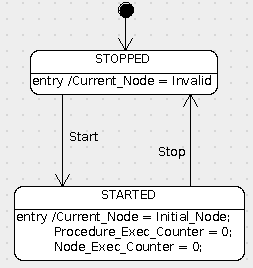
\includegraphics[scale=0.5,keepaspectratio=true]{../images/PR_StartStop.png}
 \caption{Procedure Start/Stop Behaviour}
 \label{fig:PrStartStop}
\end{figure}
%======================================================================================

%======================================================================================
\subsection{Execution Requirements}\label{req:execInterface}
%======================================================================================

\begin{fw_req_note}{Execution Interface}{T}
%----------------------------------------------------------------------------
{The C1 Implementation shall provide an interface through which a procedure 
can be executed.}
%-----------------------------------------------------------------------------
{A procedure is executed by sending an "Execute" command to it.}
%-----------------------------------------------------------------------------
{The executability of a procedure is defined by the FW Profile. 
The intended use of the C1 Implementation is to support the implementation of the procedure 
concept of the FW Profile.}
%-----------------------------------------------------------------------------
{The execution interface is implemented in \texttt{FwPrCore.h} by 
function \texttt{FwPrExecute}.} 
%-----------------------------------------------------------------------------
{The Test Cases in the Test Suite send execution commands to procedures 
through the functions of the \texttt{FwPrCore.h} module and this module has 100\% coverage.}
%----------------------------------------------------------------------------
\end{fw_req_note}


\begin{fw_req}{Execution Behaviour}{T}
%----------------------------------------------------------------------------
{The C1 Implementation shall implement the execution behaviour defined in the 
activity diagram of Figure \ref{fig:PrExecuting}.}
%-----------------------------------------------------------------------------
{The activity diagram of Figure \ref{fig:PrExecuting} is the same as the activity diagram which defines the execution behaviour in the FW Profile definition of \cite{ref:fwprofile}.}
%-----------------------------------------------------------------------------
{The execution behaviour is implemented in function \texttt{FwPrExecute}.} 
%-----------------------------------------------------------------------------
{The verification of this requirement is done in appendix 
\ref{Appendix_D_PR_Exec} where it is shown that every branch of the activity diagram of Figure 
\ref{fig:PrExecuting} is covered by at least one Test Case in the Test Suite.}
%----------------------------------------------------------------------------
\end{fw_req}

%======================================================================================
\begin{figure}[h]
 \centering
 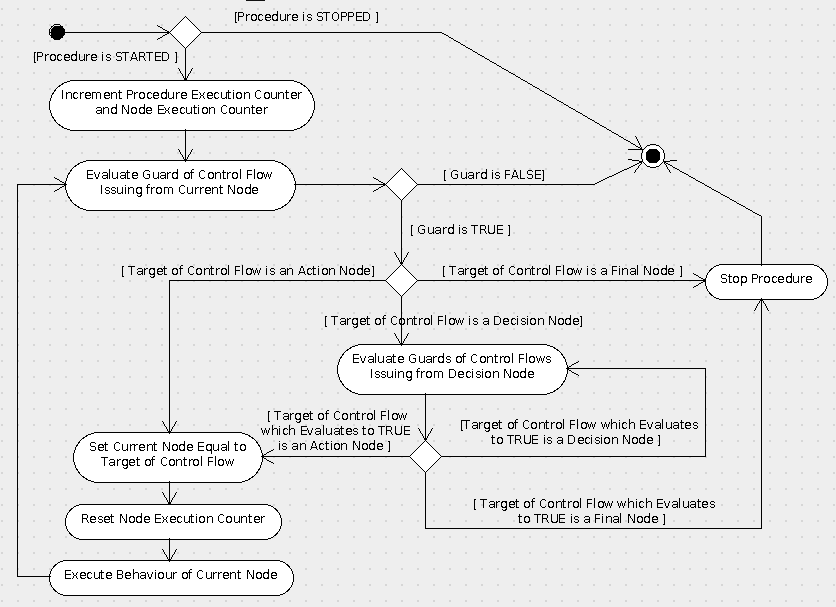
\includegraphics[scale=0.4,keepaspectratio=true]{../images/PR_Execution.png}
 \caption{Procedure Execution Logic}
 \label{fig:PrExecuting}
\end{figure}
%======================================================================================

\newpage

%------------{Order of Evaluation of Guards}
\begin{fw_req_note}{Order of Evaluation of Guards}{T}
%----------------------------------------------------------------------------
{If processing of an execution request requires evaluation of several control flow guards associated to different control flows out of the same decision node, then the control flow guards shall be evaluated in the order in which their control flows have been added to the procedure during the procedure configuration process.}
%-----------------------------------------------------------------------------
{Control flows are "added" to a procedure during the procedure configuration process.
This requirement assumes that they are added in sequence and one by one.}
%-----------------------------------------------------------------------------
{In principle, if the guards on the control flows out of a decision node are mutually exclusive and do not have side effects, their order of evaluation is irrelevant. 
For this reason, the FW Profile of \cite{ref:fwprofile} does not specify the order of evaluation of control flow guards.
However, in embedded applications with constrained CPU and memory resources, determinism in the order of evaluation may be exploited to improve run-time efficiency (for instance, by ensuring that the guard which is most likely to be true is evaluated first) and to implement "else" clauses in an efficient manner (see section 4.6 of \cite{ref:um}).}
%-----------------------------------------------------------------------------
{The evaluation of the guards on the control flows out of a decision node is done in function \texttt{FwPrExecute}.} 
%-----------------------------------------------------------------------------
{The order of evaluation of control flow guards is verified in test case \texttt{FwPrTestCaseExecute9}.}
%----------------------------------------------------------------------------
\end{fw_req_note}


\begin{fw_req}{Change of Internal State}{T}
%----------------------------------------------------------------------------
{After having been completely and successfully configured, a procedure shall 
only ever change its internal state either in response to a Start/Stop command or in response to 
an Execute Command.}
%-----------------------------------------------------------------------------
{The procedure model of the FW Profile stipulates that the internal state 
of a procedure can only change in response to a Start/Stop command or in response to an Execute 
Command.}
%-----------------------------------------------------------------------------
{The current state of a procedure is the node at which the procedure is 
waiting.
The only functions in \texttt{FwPrCore.h} which can change the current state of a procedure 
are: \texttt{FwPrStart}, \texttt{FwPrStop}, and \texttt{FwPrExecute}. 
These are precisely the functions which implement the Start/Stop behaviour and the response to a 
Transition Command.} 
%-----------------------------------------------------------------------------
{A search for \texttt{curNode} (the field of the PRD which holds the 
current node) in the \texttt{FwPrCore.c} file shows that this attribute is assigned to in only 
the following functions: \texttt{FwPrStart}, \texttt{FwPrStop}, and \texttt{FwPrExecute}.}
%----------------------------------------------------------------------------
\end{fw_req}


\begin{fw_req}{Dynamical Constraint}{T}
%----------------------------------------------------------------------------
{The C1 Implementation shall check compliance with the dynamical constraint 
D1 defined in section 4.2 of the FW Profile Definition in \cite{ref:fwprofile}.}
%-----------------------------------------------------------------------------
{The D1 constraint represents a non-nominal situation which cannot be detected statically. 
The C1 Implementation targets mission critical applications where the ability to detect non-
nominal situations is important to guarantee the integrity of a system.}
%-----------------------------------------------------------------------------
{The check for the D1 condition is implemented in the 
\texttt{FwPrExecute} function. 
Its detection results in error \texttt{prFlowErr}.} 
%-----------------------------------------------------------------------------
{Test Case \texttt{FwPrTestCaseCheck4} simulates a situation where error 
\texttt{prFlowErr} is reported because execution of a transition through a decision node finds 
that all out-going control flows have guards which evaluate to false.}
%----------------------------------------------------------------------------
\end{fw_req}


\begin{fw_req}{Procedure Data}{T}
%----------------------------------------------------------------------------
{As part of the processing of an execution request to a procedure, 
it shall be possible to exchange data with the actions and guards of the procedure.}
%-----------------------------------------------------------------------------
{The FW Profile stipulates that execution commands may carry data.}
%-----------------------------------------------------------------------------
{Function \texttt{FwPrExecute} in \texttt{FwPrCore.h} implements the 
code through which the actions of a procedure are executed and its guards are evaluated. 
These functions pass the PRD to the functions implementing the procedure actions and procedure 
guards. 
In the PRD, field \texttt{prData} is reserved to hold a pointer to a generic data structure. 
This data structure is intended to hold the data which are exchanged with the actions and guards 
of a procedure.} 
%-----------------------------------------------------------------------------
{The Test Procedures used in the Test Cases use an instance of 
\texttt{struct TestPrData} as the means to exchange data with the actions and guards of a 
procedures. 
For example, the Test Cases \texttt{FwPrTestCaseExecute*} use this data structure to keep 
track of which actions are executed during a test.}
%----------------------------------------------------------------------------
\end{fw_req}


\begin{fw_req}{Procedure State}{T}
%----------------------------------------------------------------------------
{It shall be possible to read the current state of a procedure.}
%-----------------------------------------------------------------------------
{Applications need to be able to check the state of a procedure.}
%-----------------------------------------------------------------------------
{The state of a procedure is determined by its Stopped/Started state and 
by its current node.
Read-only access to the current node of a procedure is provided by function 
\texttt{FwPrGetCurNode}. 
Function \texttt{FwPrIsStarted} checks whether a procedure has been started.} 
%-----------------------------------------------------------------------------
{Function \texttt{FwPrGetCurNode} is used in virtually all Test Cases of 
the Test Suite. 
Function \texttt{FwPrIsStarted} is used in, for instance, Test Case \texttt{FwPrTestCaseExecute8}.}
%----------------------------------------------------------------------------
\end{fw_req}

%======================================================================================
\subsection{Error Handling Requirements}\label{req:errorCodePR}
%======================================================================================

\begin{fw_req}{Error Code}{T}
%----------------------------------------------------------------------------
{The PRD shall store the code of the last error encountered during the PRD 
configuration process or during the processing of execution requests.}
%-----------------------------------------------------------------------------
{The C1 Implementation targets embedded mission-critical applications 
where there normally is a need to periodically monitor the integrity of an application. 
The embedded character of the application, however, also means that memory resources are often 
limited and it may consequently not be possible to maintain a log of all errors. 
This requirement represents a compromise between these two needs in the sense that it allows an 
application to check whether an error has occured with only minimal storage requirements.}
%-----------------------------------------------------------------------------
{The error code is stored in field \texttt{errCode} of the PRD.} 
%-----------------------------------------------------------------------------
{The Test Cases with names like \texttt{FwPrTestCaseCheck*} test various 
error conditions and verify that the most recent error condition is correctly stored in the error 
code of an PRD. 
Appendix \ref{Appendix_B_Error_Checks} lists the configuration and dynamic errors which may be 
reported in the error code of a PRD and, for each error, it identifies a Test Case where that 
error is reported and verified.}
%----------------------------------------------------------------------------
\end{fw_req}


\begin{fw_req}{Access to Error Code}{T}
%----------------------------------------------------------------------------
{The PRD shall provide read-only access to the error code.}
%-----------------------------------------------------------------------------
{See the justification of the previous requirement.}
%-----------------------------------------------------------------------------
{The value of the error code can be read with function 
\texttt{FwPrGetErrCode}.} 
%-----------------------------------------------------------------------------
{See verification of the previous requirement.}
%----------------------------------------------------------------------------
\end{fw_req}


%======================================================================================
\subsection{Derived Procedure Creation Requirements}
%======================================================================================

\begin{fw_req}{Extension Interface}{T}
%----------------------------------------------------------------------------
{The C1 Implementation shall provide an interface through which the PRD of a \emph{derived procedure} can be created from the PRD of a \emph{base procedure}.}
%-----------------------------------------------------------------------------
{The FW Profile defines an \emph{adaptation mechanism} through which a new procedure can be built 
from an existing procedure by selectively modifying some of its elements. The extension mechanism of the C1 Implementation is an 
implementation of this adaptation mechanism.}
%-----------------------------------------------------------------------------
{The procedure extension interface is implemented alongside the procedure creation interface in 
modules \texttt{FwPrDCreate.h} and \texttt{FwPrSCreate.h}.} 
%-----------------------------------------------------------------------------
{In the test suite, derived procedures are used. The derived procedures are created in functions 
\texttt{FwPrMakeTestPRDer1} and \texttt{FwPrMakeTestPRDer1Static}. These make functions exercise all derived PRD creation functions offered 
by the C1 Implementation.}
%----------------------------------------------------------------------------
\end{fw_req}


\begin{fw_req_note}{Dynamic and Static Derived PRD Creation}{T}
%----------------------------------------------------------------------------
{It shall be possible to create the PRD of a derived procedure either statically or dynamically.}
%-----------------------------------------------------------------------------
{The term \emph{static} refers to an instantiation process which does not rely on dynamic memory
allocation.}
%-----------------------------------------------------------------------------
{Dynamic creation of a derived procedure is convenient, but may be forbidden in mission-critical applications.}
%-----------------------------------------------------------------------------
{Dynamic creation of a derived procedure is defined in \texttt{FwPrDCreate.h}. 
Static creation of a derived procedure creation is defined in \texttt{FwPrSCreate.h}.} 
%-----------------------------------------------------------------------------
{In the Test Suite, derived procedures are used. A derived procedure is created dynamically in 
function \texttt{FwPrMakeTestPRDer1} and statically in function \texttt{FwPrMakeTestPRDer1Static}.}
%----------------------------------------------------------------------------
\end{fw_req_note}


\begin{fw_req}{Release of Derived PRD}{T}
%----------------------------------------------------------------------------
{If the PRD of a derived procedure is created dynamically, then it shall also be possible to destroy it dynamically by releasing the memory that was allocated to it.}
%-----------------------------------------------------------------------------
{The target applications for the C1 Implementation are mission-critical applications. In this domain, dynamic memory allocation is only allowed if the means are available to reclaim the dynamically allocated memory.}
%-----------------------------------------------------------------------------
{Function \texttt{FwPrReleaseDer} is provided in \texttt{FwPrDCreate.h} to release the memory allocated when a new derived PRD is created dynamically.} 
%-----------------------------------------------------------------------------
{Test Cases \texttt{FwPrTestCaseDer1} and \texttt{FwPrTestCaseDer2},
manipulate derived procedures whose PRD is created dynamically. 
The memory used by these PRDs is released before the end of the test. 
In the Acceptance Test for the C1 Implementation (see \cite{ref:um}, the Test Suite is run 
with the Valgrind tool and it is verified that no memory leaks occur and 
that all memory allocated dynamically is then released in an orderly way.}
%----------------------------------------------------------------------------
\end{fw_req}


\begin{fw_req_note}{Time of Derived PRD Creation}{T}
%----------------------------------------------------------------------------
{It shall be possible to create a derived procedure from a base procedure at any time after the base procedure has been fully and correctly configured.}
%-----------------------------------------------------------------------------
{This requirement in particular implies that procedure extension can be done on procedures which have already been started.}
%-----------------------------------------------------------------------------
{This requirement complements the requirement allowing dynamic creation of derived procedures: the intention behind 
both requirements is to allow an application to create a new derived procedure at any time and under any circumstances.}
%-----------------------------------------------------------------------------
{Function \texttt{FwPrCreateDer} which creates the PRD for a new derived procedure performs no check on the state of the 
base procedure (but, if the base procedure is not fully and correctly configured, the behaviour of the derived procedure is undefined).} 
%-----------------------------------------------------------------------------
{Test Cases \texttt{FwPrTestCaseDer1} and \texttt{FwPrTestCaseDer2}
manipulate derived procedures whose PRD is created dynamically. 
Test Case \texttt{FwPrTestCaseDer1} derives the new PRD from a base procedure which has not yet been started 
whereas Test Case \texttt{FwPrTestCaseDer2} 
derives it from a base procedure which has already been started and executed.}
%----------------------------------------------------------------------------
\end{fw_req_note}


\begin{fw_req_note}{Configuration of Derived PRD at Creation}{T}
%----------------------------------------------------------------------------
{After successful creation, the PRD of a derived procedure shall be a structural clone of the PRD of the base procedure.}
%-----------------------------------------------------------------------------
{The expression \emph{structural clone} must be understood as follows. Procedure B is a structural clone of procedure A if the following conditions are satisfied: A has the same action nodes with the same actions as B; A has the decision nodes as B; A has the same control flows between the same nodes and with the same guards as B.}
%-----------------------------------------------------------------------------
{The procedure extension mechanism is intended to represent the procedure adaptation mechanism of the FW Profile. 
The adaptation mechanism of FW Profile is implemented in the C1 Implementation through a 2-step process: first, a clone of the base procedure is 
obtained by extending the base procedure and then selected elements of the derived procedure are overridden. This implementation of the adaptation 
mechanism therefore requires that a newly derived procedure be a clone for all its structural elements of the base procedure.}
%-----------------------------------------------------------------------------
{The PRD (i.e. the \texttt{struct FwPrDesc}) is internally split into two parts: the \emph{extension descriptor} and the 
\emph{base descriptor}. The base descriptor holds the information about the topology of a procedure (its action nodes and decision nodes and 
their inter-connections). The extension descriptor holds the information about the actions and guards. The base descriptor 
is shared between a base procedure and its derived procedures. Hence, a derived procedure is guaranteed by design to have the same topology 
as its base procedure. The equality of the guards and actions  
is implemented in the \texttt{FwPrCreateDer} function (for the case of dynamic procedure extension) and in the \texttt{FwPrInitDer} function 
(for the case of static procedure extension).} 
%-----------------------------------------------------------------------------
{Test Case \texttt{FwPrTestCaseDerCheck1} verifies that a derived procedure and 
its base procedure are structural clones of each other both for the case of dynamic and for the case of 
static procedure extension.}
%----------------------------------------------------------------------------
\end{fw_req_note}


\begin{fw_req}{State of Derived PRD at Creatio}{T}
%----------------------------------------------------------------------------
{After successful creation, the PRD of a derived procedure shall be in the Stopped state.}
%-----------------------------------------------------------------------------
{This requirement enhances determinism of behaviour and determinism of behaviour is important in mission-critical applications.}
%-----------------------------------------------------------------------------
{The initial state of a derived procedure is set in the \texttt{FwPrCreateDer} function (for the case of dynamic procedure 
extension) and in the \texttt{FwPrInitDer} function (for the case of static procedure extension).} 
%-----------------------------------------------------------------------------
{Test Case \texttt{FwPrTestCaseDerCheck3} verifies that a dynamically 
derived procedure is in the Stopped state at creation.
Test Case \texttt{FwPrTestCaseDerCheck5} does the same for a statically derived procedure.}
%-----------------------------------------------------------------------------
\end{fw_req}


\begin{fw_req}{Error Code of Derived PRD at Creation}{T}
%-----------------------------------------------------------------------------
{After successful creation, the error code of a derived procedure shall be the same as the error code of the base procedure.}
%-----------------------------------------------------------------------------
{Extension of a procedure should only be done if the base procedure is correctly and fully configured (namely if no errors are reported by its error code). 
If this constraint is not satisfied, then the derived procedure cannot be assumed to be properly configured. 
The fact that its error code is the same as the (non-nominal) error code of its base procedure makes it easier for an application to detect the problem.}
%-----------------------------------------------------------------------------
{The initial value of the error code of a derived procedure is set in the \texttt{FwPrCreateDer} function (for the case of dynamic procedure extension) and in the \texttt{FwPrInitDer} function (for the case of static procedure extension).} 
%-----------------------------------------------------------------------------
{Test Case \texttt{FwPrTestCaseDerCheck3} verifies that a dynamically 
derived procedure has the same error code as its base procedure.
Test Case \texttt{FwPrTestCaseDerCheck5} does the same for a statically derived procedure.}
%-----------------------------------------------------------------------------
\end{fw_req}

%======================================================================================
\subsection{Derived Procedure Configuration Requirements}\label{req:configInterfaceDerivedPR}
%======================================================================================

\begin{fw_req}{Action Override}{T}
%-----------------------------------------------------------------------------
{After a derived procedure has been successfully created, it shall be possible to override one or more of its actions 
with a new action (\emph{action override operation}).}
%-----------------------------------------------------------------------------
{The overriding of an action is one of the adaptation mechanisms mandated by the FW Profile.}
%-----------------------------------------------------------------------------
{The action override operation is implemented by function \texttt{FwPrOverrideAction} in \texttt{FwPrConfig.h}.} 
%-----------------------------------------------------------------------------
{The action override mechanism is used in the Test Procedure \texttt{PR1Der} created by function 
\texttt{FwPrMakeTestPRDer1} (dynamic creation) and \texttt{FwPrMakeTestPRDer1Static} (static creation). This Test Procedure is used in 
Test Cases \texttt{FwPrTestCaseDer2} (dynamic creation) and \texttt{FwPrTestCaseDer3} (static creation).}
%-----------------------------------------------------------------------------
\end{fw_req}


%======================================================================================


\begin{fw_req_note}{Overridden Action}{T}
%-----------------------------------------------------------------------------
{The execution of the \emph{action override operation} shall require knowledge of the identity of the overridden action.}
%-----------------------------------------------------------------------------
{This requirement implies that it must not be possible to specify that a derived PRD overrides the action of a certain 
node in the base procedure. This must only be possible if the name of the overridden action is known.}
%-----------------------------------------------------------------------------
{Ideally, it would be desirable to have a mechanism through which a base procedure can declare that certain actions 
are "final" and cannot therefore be overridden. Implementation of such a mechanism is judged too onerous in terms of memory and CPU requirements 
and is therefore regarded as unsuitable for an implementation aimed at embedded applications (which are often memory- and CPU-constrained). 
This requirement implies a more limited mechanism through which a base procedure can protect its actions from being overridden by keeping 
their identity private.}
%-----------------------------------------------------------------------------
{Function \texttt{FwPrOverrideAction} requires as an argument the name of the function which implements the actions to be overridden.} 
%-----------------------------------------------------------------------------
{Function \texttt{FwPrOverrideAction} requires as an argument the name of the function which implements the action to be overridden. 
Hence, an action can be overridden only if the name of the function implementing it is in scope. A base procedure can therefore prevent one of its actions 
from being overridden by keeping the function that implements it hidden (for instance, by declaring it as a \texttt{static} function).}
%-----------------------------------------------------------------------------
\end{fw_req_note}


%======================================================================================


\begin{fw_req}{Guard Override}{T}
%-----------------------------------------------------------------------------
{After a derived procedure has been successfully created, it shall be possible to override one or more of its guards with 
a new guard (\emph{guard override operation}).}
%-----------------------------------------------------------------------------
{The overriding of a guard is one of the adaptation mechanisms mandated by the FW Profile.}
%-----------------------------------------------------------------------------
{The guard override operation is implemented by function \texttt{FwPrOverrideGuard} in \texttt{FwPrConfig.h}.} 
%-----------------------------------------------------------------------------
{The guard override mechanism is used in the Test Procedure \texttt{PR1Der} created by function 
\texttt{FwPrMakeTestPRDer1} (dynamic creation) and \texttt{FwPrMakeTestPRDer1Static} (static creation). This Test Procedure is used in 
Test Cases \texttt{FwPrTestCaseDer2} (dynamic creation) and \texttt{FwPrTestCaseDer3} (static creation).}
%-----------------------------------------------------------------------------
\end{fw_req}


%======================================================================================


\begin{fw_req_note}{Overridden Guard}{T}
%-----------------------------------------------------------------------------
{The execution of the \emph{guard override operation} shall require knowledge of the identity of the overridden guard.}
%-----------------------------------------------------------------------------
{This requirement implies that it must not be possible to specify that a derived PRD overrides, say, the guard of a certain control flow in the base procedure. 
This must only be possible if the name of the overridden guard is known.}
%-----------------------------------------------------------------------------
{Ideally, it would be desirable to have a mechanism through which a base procedure can declare that certain guards 
are "final" and cannot therefore be overridden. Implementation of such a mechanism is judged too onerous in terms of memory and CPU requirements 
and is therefore regarded as unsuitable for an implementation aimed at embedded applications (which are often memory- and CPU-constrained). 
This requirement implies a more limited mechanism through which a base procedure can protect its guards from being overridden by keeping 
their identity private.}
%-----------------------------------------------------------------------------
{Function \texttt{FwPrOverrideGuard} requires as an argument the name of the function which implements the guards to be overridden.} 
%-----------------------------------------------------------------------------
{Function \texttt{FwPrOverrideGuard} requires as an argument the name of the function which implements the guards to be overridden. 
Hence, a guard can be overridden only if the name of the function implementing it is in scope. A base procedure can therefore prevent one of its guards 
from being overridden by keeping the function that implements it hidden (for instance, by declaring it as a \texttt{static} function).}
%-----------------------------------------------------------------------------
\end{fw_req_note}



%=============================================================================
\section{RT Containers - Functional Requirements}\label{sec:rtFncReqs}
This section defines the functional requirements for the RT Container part of the C1 Implementation. The functional requirements are those which define the functional behaviour of the RT containers in the C1 Implementation.

%=============================================================================

\begin{fw_req}{Implementation of RT Container Concept}{R}
{The C1 Implementation shall implement the RT container concept of the FW Profile of \cite{ref:fwprofile}.}
%-----------------------------------------------------------------------------
{The intended use of the C1 Implementation is to support the implementation of the RT container concept of the FW Profile.}
%-----------------------------------------------------------------------------
{The RT container behaviour specified by the FW Profile is implemented by the \texttt{FwRtCore.h} interface of the C1 Implementation.} 
%-----------------------------------------------------------------------------
{The FW Profile defines RT containers in terms of their \emph{elements} 
and of their \emph{behaviour}. The container behaviour is in turn defined in terms of the behaviour of two procedures, of one thread, and of the three operations which can be performed upon a container (\texttt{Start}, \texttt{Stop}, and \texttt{Notify}). Appendix \ref{Appendix_A_Implementation_RT_Concept} shows how the container elements and the container operations are mapped to data structures and functions in the C1 Implementation}
\end{fw_req}


%======================================================================================
\subsection{RT Container Descriptor (RTD) Requirements}\label{req:RTD}
%======================================================================================

\begin{fw_req}{RT Container Descriptor (RTD)}{R}
%----------------------------------------------------------------------------
{It shall be possible to address and to manipulate a RT Container as a single entity (the \emph{RT Container Descriptor} or RTD).}
%-----------------------------------------------------------------------------
{The intended use of the C1 Implementation is to provide modules which can be deployed within another application. The definition of the RTD simplifies the interface between the modules of the C1 Implementation and the user application.}
%-----------------------------------------------------------------------------
{The RTD is defined by type \texttt{struct FwRtDesc}.} 
%-----------------------------------------------------------------------------
{A RT container is represented by an instance of type \texttt{struct FwRtDesc} and is manipulated as an instance of type \texttt{FwRtDesc\_t}. All functions which operate on a RT container take an instance of this type as their argument.}
%----------------------------------------------------------------------------
\end{fw_req}


\begin{fw_req}{RTD Encapsulation}{R}
%----------------------------------------------------------------------------
{The RTD shall encapsulate all the information defining the configuration and the current state of its container.}
%-----------------------------------------------------------------------------
{The intended use of the C1 Implementation is to provide modules which can be deployed within another application. The encapsulation of all information related to a RT container in a single data structure simplifies the interface between the modules of the C1 Implementation and the user application.}
%-----------------------------------------------------------------------------
{The RTD is defined as an instance of type \texttt{struct FwRtDesc}.} 
%-----------------------------------------------------------------------------
{The configuration information for a container is defined through the operations of \texttt{FwRtConfig.h}. These operation only manipulate the RTD. The state of a container is defined by the value of its Notification Counter and by the container state. These are mapped to fields \texttt{notifCounter} and \texttt{state} in the RTD.}
%----------------------------------------------------------------------------
\end{fw_req}  

%======================================================================================
\subsection{Creation Requirements}\label{req:creationInterfaceRTD}
%======================================================================================

\begin{fw_req}{Creation Interface}{T}
%----------------------------------------------------------------------------
{ The C1 Implementation shall provide an interface through which a new RTD 
can be created.}
%-----------------------------------------------------------------------------
{Applications which wish to manipulate an RT container must first create the 
RTD which represents it.}
%-----------------------------------------------------------------------------
{The RTD creation interface is trivial in the sense that RTDs are created by instantiating a variable of type \texttt{struct FwRtDesc}.} 
%-----------------------------------------------------------------------------
{In every RT container test case in the test suite, one or more RTDs are created.}
%----------------------------------------------------------------------------
\end{fw_req}

\begin{fw_req_note}{Dynamic and Static Creation}{T}
%----------------------------------------------------------------------------
{ It shall be possible to create a new RTD either statically or dynamically.}
%-----------------------------------------------------------------------------
{The term \emph{static} refers to an instantiation process which does not rely on dynamic memory allocation.}
%-----------------------------------------------------------------------------
{Dynamic creation of containers is convenient but may be forbidden in mission-critical applications.}
%-----------------------------------------------------------------------------
{RTDs are created by instantiating a variable of type \texttt{struct FwRtDesc}. Applications are free to instantiate this variable either statically (on the stack or as a global variable) or dynamically (through a call to \texttt{malloc}). } 
%-----------------------------------------------------------------------------
{In every RT container test case in the test suite, one or more RTDs are created. In test case \texttt{FwRtTestCaseRunDefault1}, the RTD is created dynamically (using \texttt{malloc}); in all other test cases, the RTDs are created statically.}
%----------------------------------------------------------------------------
\end{fw_req_note}


%======================================================================================
\subsection{Configuration Requirements}\label{req:configInterfaceRTD}
%======================================================================================

\begin{fw_req}{Configuration Interface}{T}
%----------------------------------------------------------------------------
{The C1 Implementation shall provide an interface through which an RTD can be configured and made to match the characteristics of a certain RT Container.}
%-----------------------------------------------------------------------------
{Applications which wish to manipulate a RT Container must configure it before they can send notification requests to it.}
%-----------------------------------------------------------------------------
{The container configuration interface is implemented in \texttt{FwRtConfig.h}.} 
%-----------------------------------------------------------------------------
{In the test suite, test RT containers are configured. The Test Suite exercises all configuration functions in \texttt{FwRtConfig.h} (it has 100\% statement coverage of the implementation of this interface with the exception of code which is entered when a POSIX system call fails).}
%----------------------------------------------------------------------------
\end{fw_req}


\begin{fw_req_note}{Reconfiguration of an RTD}{T}
%----------------------------------------------------------------------------
{It shall not be possible to re-configure an RTD dynamically while it is being used to process notification requests.}
%-----------------------------------------------------------------------------
{The term \textit{configuration} refers to the operations which must be performed on a newly-created RTD before it can be started.}
%-----------------------------------------------------------------------------
{ The C1 Implementation targets mission-critical applications. In this domain, dynamic reconfiguration of RT containers would be regarded as unsafe because it makes it harder to determine behaviour through static analysis.}
%-----------------------------------------------------------------------------
{ The RTD configuration functions (with the exception of the \texttt{FwRtReset} function and of the \texttt{FwRtSetData} function) check the container state and are only effective if the container is in state \texttt{rtContUninitialized}. In all other cases (i.e. during the container's operational use), they cause an error state to be entered. No such check is possible for the \texttt{FwRtReset} function because the purpose of this function is precisely to initialize the RTD and therefore no assumption can be made about the RTD state at the time the function is called. No such check is needed for the \texttt{FwRtSetData} function because the purpose of this function is to load the container data and this is an optional operation.  } 
%-----------------------------------------------------------------------------
{ Test Case \texttt{FwRtTestCaseSetAction1} verifies that attempts to load a new container procedure action or to re-initialize the container during the container's operational phase lead to an error. Test Case \texttt{FwRtTestCaseSetAttr1} verifies that attempts to load a new POSIX attribute obect during the container's operational phase lead to an error.}
%----------------------------------------------------------------------------
\end{fw_req_note}


\begin{fw_req}{Setting of POSIX Attributes}{T}
%----------------------------------------------------------------------------
{During the configuration process, it shall be possible to set the attributes of any POSIX object used by a RT container (see requirement FW-\ref{req:dependencyReqs}.2).}
%-----------------------------------------------------------------------------
{ The C1 Implementation targets mission-critical applications. In this domain, it is often important to fine-tune the real-time behaviour of threads. This requires access to the attributes to the POSIX objects upon which the real-time behaviour of a RT container is built.}
%-----------------------------------------------------------------------------
{ Function \texttt{FwRtSetMutexAttr} allows the POSIX attribute objects of a container's thread, of its mutex and of its condition variable to be set. } 
%-----------------------------------------------------------------------------
{ Test Case \texttt{FwRtTestCaseRunNonNullAttr1} verifies that it is possible to load non-NULL attributes for the POSIX thread, the POSIX mutex and the POSIX condition variable associated to a RT container.}
%----------------------------------------------------------------------------
\end{fw_req}

\subsection{Start and Stop Requirements}\label{req:startStopInterfaceRTD}
%======================================================================================

\begin{fw_req}{Start and Stop Interface}{T}
%----------------------------------------------------------------------------
{ The C1 Implementation shall provide an interface through which the  RT Container represented by an RTD can be started, stopped and queried for its current Started/Stopped status.}
%-----------------------------------------------------------------------------
{The Start/Stop operations are defined by the FW Profile. The intended use of the C1 Implementation is to support the implementation of the RT container concept of the FW Profile.}
%-----------------------------------------------------------------------------
{The Start/Stop operations are implemented in module \texttt{FwRtCore.h} by functions \texttt{FwRtStart} and \texttt{FwRtStop}. The status query operation is implemented by function \texttt{FwRtGetContState} which returns the current state of a container.} 
%-----------------------------------------------------------------------------
{The Test Cases in the Test Suite start and stop RT containers and query them for their status through the functions of the \texttt{FwRtCore.h} module and this module has 100\% coverage (except for branches entered in case of POSIX system call errors).}
%----------------------------------------------------------------------------
\end{fw_req}

\begin{fw_req}{Start and Stop Behaviour}{T}
%----------------------------------------------------------------------------
{The Start and Stop interface shall implement the behaviour defined in the 
activity diagrams of Figure \ref{fig:RTStartStop}.}
%-----------------------------------------------------------------------------
{The activity diagrams of Figure \ref{fig:RTStartStop} are the same as in 
the FW Profile definition of \cite{ref:fwprofile}.}
%-----------------------------------------------------------------------------
{The Start operation is implemented by function \texttt{FwRtStart}. The Stop operation is implemented by function \texttt{FwRtStop}.} 
%-----------------------------------------------------------------------------
{The verification of this requirement is done in section \ref{Appendix_C_RT_Start_Stop}.}
%----------------------------------------------------------------------------
\end{fw_req}

\begin{figure}[h]
 \centering
 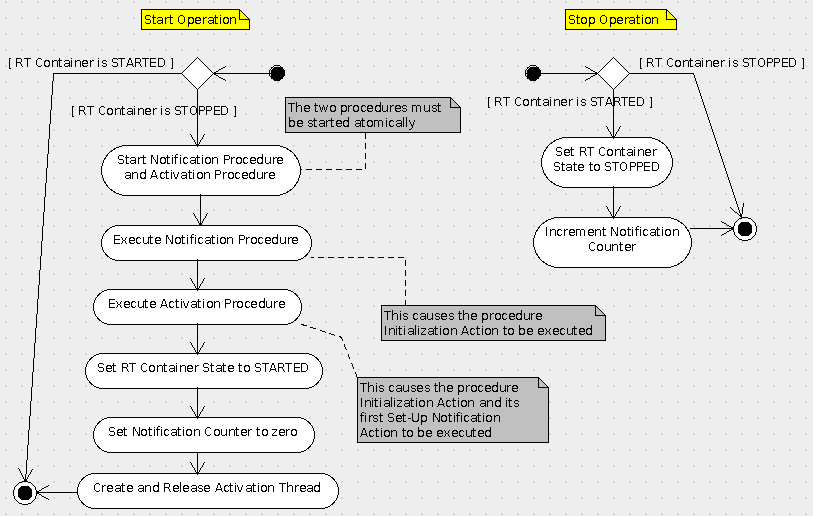
\includegraphics[scale=0.42,keepaspectratio=true]{../images/RTStartStop.png}
 \caption{RT Container Start/Stop Behaviour}
 \label{fig:RTStartStop}
\end{figure}


%======================================================================================
\subsection{Notification Requirements}\label{req:notifInterface}
%======================================================================================

\begin{fw_req}{Notification Interface}{T}
%----------------------------------------------------------------------------
{The C1 Implementation shall provide an interface through which a RT Container 
can be notified.}
%-----------------------------------------------------------------------------
{The "Notify" operation is defined by the FW Profile. The intended use of the C1 Implementation is to support the implementation of the RT container concept of the FW Profile.}
%-----------------------------------------------------------------------------
{The Notification interface is implemented in \texttt{FwRtCore.h} by 
function \texttt{FwRtNotify}.} 
%-----------------------------------------------------------------------------
{The Test Cases in the Test Suite send notification commands to RT Containers 
through the functions of the \texttt{FwRtCore.h} module and this module has 100\% coverage (except for branches entered in case of POSIX system call errors).}
%----------------------------------------------------------------------------
\end{fw_req}

\newpage 

\begin{fw_req}{Notification Behaviour}{T}
%----------------------------------------------------------------------------
{The C1 Implementation shall implement the "notify" operation to execute the Notification Procedure (see next requirement).}
%-----------------------------------------------------------------------------
{The "notify" operation is one of the three operations defined by the FW Profile. The intended use of the C1 Implementation is to support the implementation of the RT container concept of the FW Profile.}
%-----------------------------------------------------------------------------
{The notification behaviour is implemented in function \texttt{FwRtNotify}.} 
%-----------------------------------------------------------------------------
{Test Case \texttt{FwRtTestCaseRunDefault1} in the Test Suite verifies that execution of function \texttt{FwRtNotify} results in the execution of the Notification Procedure.}
%----------------------------------------------------------------------------
\end{fw_req}

\begin{fw_req}{Notification Procedure}{T}
%----------------------------------------------------------------------------
{The Notification Procedure of a RT Container shall implement the behaviour shown in the activity diagram in the left-hand side of figure \ref{fig:RTContainer}.}
%-----------------------------------------------------------------------------
{The activity diagram of figure \ref{fig:RTContainer} is the same as in the FW Profile definition.}
%-----------------------------------------------------------------------------
{The implementation of the notification procedure is split into two locations: (a) the initialization part (up to the first decision node) is implemented in function \texttt{FwRtStart} where the procedure is started and then executed for the first time; (b) the loop is implemented in function \texttt{ExecNotifProcedure} in module \texttt{FwRtCore.c}.} 
%-----------------------------------------------------------------------------
{Verification of this requirement is done in appendix \ref{Appendix_E_RT_Notif} where it is shown that every branch of the activity diagram of figure \ref{fig:RTContainer} is covered by at least one Test Case in the Test Suite.}
%----------------------------------------------------------------------------
\end{fw_req}

\begin{fw_req}{Activation Procedure}{T}
%----------------------------------------------------------------------------
{A RT Container shall implement an Activation Procedure with the behaviour shown in the activity diagram in the right-hand side of figure \ref{fig:RTContainer}.}
%-----------------------------------------------------------------------------
{The activity diagram of figure \ref{fig:RTContainer} is the same as in the FW Profile definition.}
%-----------------------------------------------------------------------------
{The implementation of the activation procedure is split into two locations: (a) the initialization part (up to the first decision node) is implemented in function \texttt{FwRtStart} where the procedure is started and then executed for the first time; (b) the loop is implemented in function \texttt{ExecActivProcedure} in module \texttt{FwRtCore.c}.} 
%-----------------------------------------------------------------------------
{Verification of this requirement is done in appendix \ref{Appendix_E_RT_Notif} where it is shown that every branch of the activity diagram of figure \ref{fig:RTContainer} is covered by at least one Test Case in the Test Suite.}
%----------------------------------------------------------------------------
\end{fw_req}


\begin{fw_req}{Activation Thread}{T}
%----------------------------------------------------------------------------
{A RT Container shall encapsulate a thread (the "Activation Thread") to execute the behaviour shown in listing \ref{code:pseudoCodeActivationThread}.}
%-----------------------------------------------------------------------------
{The behaviour shown in listing \ref{code:pseudoCodeActivationThread} is the same as the behaviour defined in reference \cite{ref:fwprofile} for the Activation Thread. }
%-----------------------------------------------------------------------------
{The Activation Thread behaviour is implemented in function \texttt{ExecActivThread} in module \texttt{FwRtCore.c}.} 
%-----------------------------------------------------------------------------
{Verification of this requirement is done in appendix \ref{Appendix_E_RT_Notif} where it is shown that every branch of the pseudo-code in listing \ref{code:pseudoCodeActivationThread} is covered by at least one Test Case in the Test Suite.}
%----------------------------------------------------------------------------
\end{fw_req}

\lstset{language=C,caption={Pseudo-code of Activation Thread},label=code:pseudoCodeActivationThread}
\begin{lstlisting}
while true do {
  wait until Notification Counter is greater than 0;
  decrement Notification Counter;
  execute Activation Procedure;
  
  if (Activation Procedure has terminated) then {
    put RT Container in STOPPED state;
    execute Notification Procedure;
    break;
  }

  if (RT Container is in state STOPPED) then {
    execute Activation Procedure;
    execute Notification Procedure;
    break;
  }
}
\end{lstlisting}


%======================================================================================
\begin{figure}[H]
 \centering
 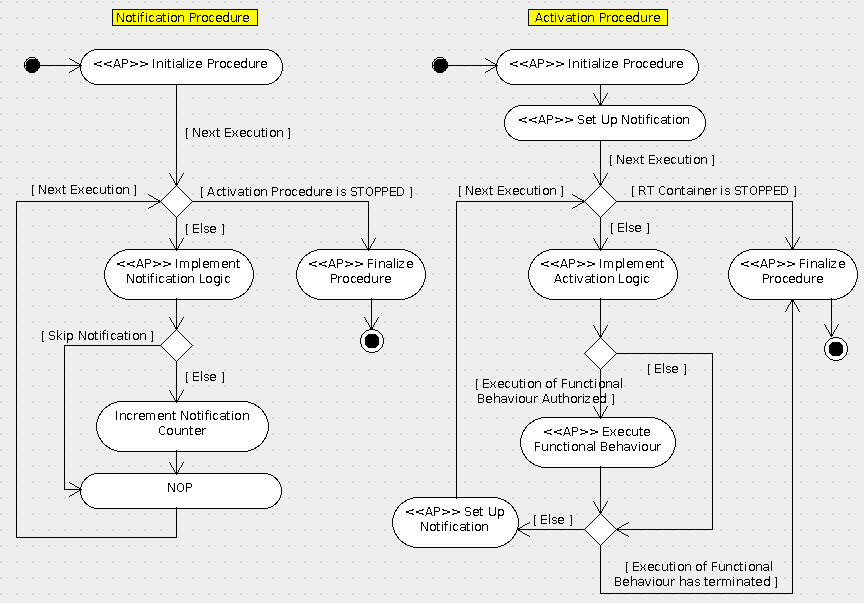
\includegraphics[scale=0.4,keepaspectratio=true]{../images/RTContainer.png}
 \caption{Notification and Activation Procedures}
 \label{fig:RTContainer}
\end{figure}
%======================================================================================

\begin{fw_req}{Wait for Activation Thread Termination}{T}
%----------------------------------------------------------------------------
{The C1 Implementation shall offer a function to let a user wait for the termination of a container's Activation Thread.}
%-----------------------------------------------------------------------------
{One of the usage constraints of a RT Container (see list in table of section 5.4 of reference \cite{ref:fwprofile}) requires that a container only be re-started after its Activation Thread has terminated. It is therefore convenient to have a function which waits until the Activation Thread has terminated execution. }
%-----------------------------------------------------------------------------
{Function \texttt{FwRtWaitForTermination} in module \texttt{FwRtCore.h} implements a blocking wait for the termination of the Activation Thread of a RT container.} 
%-----------------------------------------------------------------------------
{Function \texttt{FwRtWaitForTermination} is verified in, among others, the following Test Cases of the Test Suite: \texttt{FwRtTestCaseRunDefault1}, \texttt{FwRtTestCaseRunNonNullAttr1}, and \texttt{FwRtTestCaseStressRun1}.}
%----------------------------------------------------------------------------
\end{fw_req}

%======================================================================================
\subsection{Access Requirements}\label{req:access}
%======================================================================================

\begin{fw_req}{Access to Activation Procedure}{R}
%----------------------------------------------------------------------------
{A RT Container shall not allow its users to perform start/stop/execute operations on its Activation Procedure.}
%-----------------------------------------------------------------------------
{The properties guaranteed by a RT Container (see list in table of section 5.4 of reference \cite{ref:fwprofile}) are conditional upon the container's user not having access to the Activation Procedure. }
%-----------------------------------------------------------------------------
{The \texttt{FwRtCore.h} module does not offer any wrapper functions for starting, stopping, or executing the Activation Procedure (but note that the user has access to the procedure descriptor through the RTD).} 
%-----------------------------------------------------------------------------
{See requirement implementation.}
%----------------------------------------------------------------------------
\end{fw_req}

\begin{fw_req}{Access to Notification Procedure Start/Stop}{R}
%----------------------------------------------------------------------------
{A RT Container shall not allow its users to perform start/stop operations on its Notification Procedure.}
%-----------------------------------------------------------------------------
{The properties guaranteed by a RT Container (see list in table of section 5.4 of \cite{ref:fwprofile}) are conditional upon the container's user not having access to the start/stop interface of the Notification Procedure. }
%-----------------------------------------------------------------------------
{The \texttt{FwRtCore.h} module does not offer any wrapper functions for starting or stopping the Notification Procedure (but note that the user has access to the procedure descriptor through the RTD).} 
%-----------------------------------------------------------------------------
{See requirement implementation.}
%----------------------------------------------------------------------------
\end{fw_req}

\begin{fw_req}{Access to Notification Procedure Execution}{R}
%----------------------------------------------------------------------------
{A RT Container shall not allow its users to execute its Notification Procedure other than through the Notify operation.}
%-----------------------------------------------------------------------------
{The properties guaranteed by a RT Container (see list in table of section 5.4 of \cite{ref:fwprofile}) are conditional upon the container's user not having access to the execute interface of the Notification Procedure other than through the Notify operation. }
%-----------------------------------------------------------------------------
{The \texttt{FwRtCore.h} module does not offer any wrapper function for executing the Notification Procedure other than \texttt{FwRtNotify} (but note that the user has access to the procedure descriptor through the RTD).} 
%-----------------------------------------------------------------------------
{See requirement implementation.}
%----------------------------------------------------------------------------
\end{fw_req}

%======================================================================================
\subsection{Error Handling Requirements}\label{req:errorCodeRT}
%======================================================================================

\begin{fw_req}{Error Code}{T}
%----------------------------------------------------------------------------
{The RTD shall store the code of the last error encountered during the RTD 
configuration process or during the processing of notification requests.}
%-----------------------------------------------------------------------------
{The C1 Implementation targets embedded mission-critical applications where there normally is a need to periodically monitor the integrity of an application. The embedded character of the application, however, also means that memory resources are often limited and it may consequently not be possible to maintain a log of all errors. This requirement represents a compromise between these two needs in the sense that it allows an application to check whether an error has occured with only minimal storage requirements.}
%-----------------------------------------------------------------------------
{The C1 Implementation defines both an error code (in field \texttt{errCode} of the RTD) and a set of error states (see type \texttt{FwRtState\_t}) which, taken together, identify the last error condition encountered by a RT Container.} 
%-----------------------------------------------------------------------------
{The Test Cases \texttt{FwPrTestCaseSetAttr1} and \texttt{FwPrTestCaseSetAction1} verify the reporting of error conditions arising during the configuration process of a RT container. The only other error conditions reported by a RT container are those arising when a POSIX system call is executed. These error conditions are not verified.}
%----------------------------------------------------------------------------
\end{fw_req}


\begin{fw_req}{Access to Error Code}{T}
%----------------------------------------------------------------------------
{The RTD shall provide read-only access to the error code.}
%-----------------------------------------------------------------------------
{See the justification of the previous requirement.}
%-----------------------------------------------------------------------------
{The value of the error code can be read with function \texttt{FwRtGetErrCode}. The value of the error state can be read with function \texttt{FwRtGetContState}.} 
%-----------------------------------------------------------------------------
{See verification of the previous requirement.}
%----------------------------------------------------------------------------
\end{fw_req}


%======================================================================================
\section{Non-Functional Requirements}
%======================================================================================

This section defines the non-functional requirements of the C1 Implementation. Non-functional requirements impose overall constraints on the use, 
design, or implementation of the C1 Implementation.

%======================================================================================
\stdsubsection{Coding Requirements}\label{req:codingReqs}
%======================================================================================

\begin{fw_req}{Implementation Language}{R}
%-----------------------------------------------------------------------------
{The C1 Implementation shall be implemented in the C language.}
%-----------------------------------------------------------------------------
{The C Language is the standard language for embedded applications.}
%-----------------------------------------------------------------------------
{All the modules offered by the C1 Implementation are implemented in C.} 
%-----------------------------------------------------------------------------
{See implementation.}
%-----------------------------------------------------------------------------
\end{fw_req}


\begin{fw_req}{Compiler Warning}{T}
%-----------------------------------------------------------------------------
{The C1 Implementation shall not generate any warnings when compiled with the GCC compiler with all warnings enabled.}
%-----------------------------------------------------------------------------
{Warning may indicate weaknesses in the code or potential error.}
%-----------------------------------------------------------------------------
{See verification.} 
%-----------------------------------------------------------------------------
{The C1 Implementation Acceptance Test Procedure (see reference \cite{ref:um}) compiles all source files of the implementation using \texttt{gcc} with the option \texttt{-Wall}.}
%-----------------------------------------------------------------------------
\end{fw_req}


%======================================================================================
\subsection{Use Requirements}\label{req:userReqsSMD}
%======================================================================================

\begin{fw_req}{SMD Internal Structure}{R}
%-----------------------------------------------------------------------------
{It shall be possible to create, configure and command a state
 machine without reference to or knowledge of the internal structure of its SMD.}
%-----------------------------------------------------------------------------
{The intended use of the C1 Implementation is to provide modules 
which can be deployed within another application. 
The hiding of the information related to a state machine simplifies the interface between 
the modules of the C1 Implementation and the user application.

The target applications of the C1 Implementation are embedded applications. 
Embedded applications often have special requirements which may require changes to the internal 
structure of the SMD (perhaps to include more information about a state machine). 
This requirement would allow this to be done without affecting the interface through which 
the state machine is manipulated.} 
%-----------------------------------------------------------------------------
{See requirement verification.} 
%-----------------------------------------------------------------------------
{The functions and macros to create a state machine 
(in modules \texttt{FwSmDCreate.h} and \texttt{FwSmSCreate.h}), 
the functions to configure a state machine (in module \texttt{FwSmConfig.h}), and the 
functions to send a transition command to a state machine (in module \texttt{FwSmCore.h}) 
take as their argument a pointer to the SMD (i.e. an instance of type \texttt{FwSmDesc\_t}). 
There is therefore no need for the user to know the internal structure of the SMD to use these functions.}
%-----------------------------------------------------------------------------
\end{fw_req}

\begin{fw_req}{PRD Internal Structure}{R}
%-----------------------------------------------------------------------------
{It shall be possible to create, configure and command a procedure
 without reference to or knowledge of the internal structure of its PRD.}
%-----------------------------------------------------------------------------
{The intended use of the C1 Implementation is to provide modules 
which can be deployed within another application. 
The hiding of the information related to a procedure simplifies the interface between 
the modules of the C1 Implementation and the user application.

The target applications of the C1 Implementation are embedded applications. 
Embedded applications often have special requirements which may require changes to the internal 
structure of the PRD (perhaps to include more information about a procedure). 
This requirement would allow this to be done without affecting the interface through which 
the procedure is manipulated.} 
%-----------------------------------------------------------------------------
{See requirement verification.} 
%-----------------------------------------------------------------------------
{The functions and macros to create a procedure 
(in modules \texttt{FwPrDCreate.h} and \texttt{FwPrSCreate.h}), 
the functions to configure a procedure (in module \texttt{FwPrConfig.h}), and the 
functions to execute a procedure (in module \texttt{FwPrCore.h}) 
take as their argument a pointer to the PRD (i.e. an instance of type \texttt{FwPrDesc\_t}). 
There is therefore no need for the user to know the internal structure of the PRD to use these functions.}
%-----------------------------------------------------------------------------
\end{fw_req}

\begin{fw_req}{RTD Internal Structure}{R}
%-----------------------------------------------------------------------------
{It shall be possible to create, configure and command a RT container without reference to or knowledge of the internal structure of its RTD.}
%-----------------------------------------------------------------------------
{The intended use of the C1 Implementation is to provide modules which can be deployed within another application. The hiding of the information related to a RT container simplifies the interface between the modules of the C1 Implementation and the user application.

The target applications of the C1 Implementation are embedded applications. Embedded applications often have special requirements which may require changes to the internal
structure of the RTD (perhaps to include more information about a RT container). This requirement would allow this to be done without affecting the interface through which 
the RT container is manipulated.} 
%-----------------------------------------------------------------------------
{See requirement verification.} 
%-----------------------------------------------------------------------------
{The functions which manipulate a RT container take as their argument a pointer to the RTD (i.e. an instance of type \texttt{FwPrDesc\_t}). There is therefore no need for the user to know the internal structure of the RTD to use these functions.}
%-----------------------------------------------------------------------------
\end{fw_req}


%======================================================================================
\subsection{Resource Requirements}\label{req:resourceReqs}
%======================================================================================

\begin{fw_req_note}{Code Memory Footprint}{T}
%-----------------------------------------------------------------------------
{The code memory footprint of the C1 Implementation shall be independent of 
the size and number of state machines, procedures, and RT containers deployed by an application.}
%-----------------------------------------------------------------------------
{Ideally, it would be desirable to impose a requirement on the memory occupation 
of the C1 Implementation. 
This is not possible because memory occupation depends on the tool chain used to compile an 
application and on the target processor. 
This and the next requirement aim to restrict memory occupation in a manner which is independent of the compilation tool chain and of the execution hardware.}
{Embedded applications are often memory-constrained.}
%-----------------------------------------------------------------------------
{See requirement verification.} 
%-----------------------------------------------------------------------------
{The C1 Implementation provides a set of functions which create, 
configure and manipulate a generic state machine or procedure. 
RT containers are created by direct instantiation of a type defined by the C1 Implementation. 
There is no code generation facility (neither explicit, nor implicit through the use of macros) which generates \emph{ad hoc} code for each state machine, procedure, or RT container instance or for categories of state machines, procedures, or RT containers. 
Thus, the code base of the C1 Implementation is fixed and independent of the number 
and type of state machines, procedures and RT containers instantiated by an application.}
%-----------------------------------------------------------------------------
\end{fw_req_note}


\begin{fw_req_note}{SMD Footprint}{T}
%-----------------------------------------------------------------------------
{The theoretical memory requirement for an SMD instance shall 
be a linear function of the values of the following attributes 
of the SMD: number of states, number of choice pseudo-states, number of transitions, 
number of actions, number of guards.}
%-----------------------------------------------------------------------------
{The expression "theoretical memory requirement" refers to the memory requirement 
of an ideal compiler which packs all the items in the SMD so as to minimize its memory 
occupation (in reality, some compilers have alignment constraints which increase memory occupation).}
%-----------------------------------------------------------------------------
{Embedded applications are often memory-constrained. A linear 
dependency of the data memory requirements on the size of a state machine minimizes 
the memory requirements (it is not possible to have a less-than-linear dependency 
because different state machine instances are independent of each other).}
%-----------------------------------------------------------------------------
{The memory occupation of an SMD instance is determined by the 
internal structure of an SMD which is defined by type 
\texttt{struct FwSmDesc} in \texttt{FwSmPrivate.h}.} 
%-----------------------------------------------------------------------------
{The User Manual (see reference \cite{ref:um}) provides a formula to compute the theoretical 
memory footprint of a single SMD instance (see section "Memory Footprint"). 
This formula is linear in the number of states, number of choice 
pseudo-states, number of transitions, number of actions, 
number of guards. Note that the requirement asks for the memory footprint of an SMD to 
be proportional to the number of actions and guards in a state machine. 
This implies that, in a state machine where the same action is used at different points 
of the state machine (e.g. the same action acts as entry action of several states), one 
single function is used to implement all instances of the action.}
%-----------------------------------------------------------------------------
\end{fw_req_note}

\begin{fw_req_note}{PRD Footprint}{T}
%-----------------------------------------------------------------------------
{The theoretical memory requirement for a PRD instance shall 
be a linear function of the values of the following attributes 
of the PRD: number of action nodes, number of decision nodes, number of control flows, 
number of actions, number of guards.}
%-----------------------------------------------------------------------------
{The expression "theoretical memory requirement" refers to the memory requirement 
of an ideal compiler which packs all the items in the PRD so as to minimize its memory 
occupation (in reality, some compilers have alignment constraints which increase memory occupation).}
%-----------------------------------------------------------------------------
{Embedded applications are often memory-constrained. A linear 
dependency of the data memory requirements on the size of a procedure minimizes 
the memory requirements (it is not possible to have a less-than-linear dependency 
because different procedure instances are independent of each other).}
%-----------------------------------------------------------------------------
{The memory occupation of a PRD instance is determined by the 
internal structure of a PRD which is defined by type 
\texttt{struct FwPrDesc} in \texttt{FwPrPrivate.h}.} 
%-----------------------------------------------------------------------------
{The User Manual (see reference \cite{ref:um}) provides a formula to compute the theoretical 
memory footprint of a single PRD instance (see section "Memory Footprint"). 
This formula is linear in the number of action nodes, number of decision nodes, number of 
control flows, number of actions, 
number of guards. 
Note that the requirement asks for the memory footprint of a PRD to 
be proportional to the number of actions and guards in a procedure. 
This implies that, in a procedure where the same action is used at different points 
of the procedure (e.g. the same action is used in several action nodes), one 
single function is used to implement all instances of the action.}
%-----------------------------------------------------------------------------
\end{fw_req_note}

\begin{fw_req_note}{RTD Footprint}{T}
%-----------------------------------------------------------------------------
{The memory requirement for the part of an RTD instance directly defined by the C1 Implementation shall be independent of the characteristics of the container represented by the RTD.}
%-----------------------------------------------------------------------------
{The restriction to the "part of an RTD instance directly defined by the C1 Implementation" is necessary because an RTD also includes POSIX objects (see requirement FW-\ref{req:dependencyReqs}.2) whose memory requirements are outside the control of the C1 Implementation and cannot therefore be covered by this requirement.}
%-----------------------------------------------------------------------------
{Embedded applications are often memory-constrained. This requirement helps keep a boundary on memory requirements for RT containers (it ensures that a "large" container only uses as much memory as a "small" one).}
%-----------------------------------------------------------------------------
{The memory occupation of an RTD instance is determined by the internal structure of an RTD which is defined by type \texttt{struct FwRtDesc} in \texttt{FwRtConstants.h}.} 
%-----------------------------------------------------------------------------
{The User Manual (see reference \cite{ref:um}) provides a formula to compute the theoretical memory footprint of a single RTD instance (see section "Memory Footprint"). This formula is independent of the characterstics of the RT container. }
%-----------------------------------------------------------------------------
\end{fw_req_note}


\begin{fw_req_note}{State Machine Execution Time}{T}
%-----------------------------------------------------------------------------
{The worst-case execution time of a transition command for a
state machine shall be independent of the size of the state machine.}
%-----------------------------------------------------------------------------
{Ideally, it would be desirable to impose a requirement on the 
maximum execution time of a state machine. 
This is not possible because execution time depends on too many exogenous factors. 
This requirement aims to restrict execution time in a manner which is 
independent of the compilation/linking tool chain and execution environment.}
%-----------------------------------------------------------------------------
{Mission critical applications often need to determine 
statically the worst-case execution time of an application. 
Independence of the execution time from the size of a state machine facilitates this task.}
%-----------------------------------------------------------------------------
{Transitions in state machines are processed by function 
\texttt{FwSmMakeTrans} in module \texttt{FwSmCore.h}.} 
%-----------------------------------------------------------------------------
{Transitions for state machine are processed by function 
\texttt{FwSmMakeTrans} in module \texttt{FwSmCore.h}. 
This function executes some sequential code and then loops to evaluate the triggers 
and guards associated to all out-going transitions from the current state. 
The SMD is internally organized in such a way that it is possible to directly identify 
all out-going transitions from a given state without searching the entire set of transitions 
in the state machine. 
Thus, the maximum size of the loop in \texttt{FwSmMakeTrans} is equal to the number of out-going 
transitions from the current state. Hence, the worst-case execution time occurs when processing 
a transition from the state in a state machine which has the largest number of out-going transitions. 
The requirement is therefore satisfied if one assumes that the maximum number of out-going 
transitions from a state is bounded and independent of the size of a state machine.}
%-----------------------------------------------------------------------------
\end{fw_req_note}


\begin{fw_req_note}{Procedure Execution Time}{T}
%-----------------------------------------------------------------------------
{The worst-case time required by an execution request
to traverse a single node in a procedure shall be independent of the size of the 
procedure.}
%-----------------------------------------------------------------------------
{When a procedure is executed, zero or more nodes in the procedure
are traversed in sequence. The number of nodes thus traversed depends on the
values of the procedure guards at the time the procedure is executed.
In the absence of information about the value of the procedure guards, it is 
therefore not possible to bound the total execution time for a procedure.

Ideally, it would be desirable to impose a requirement on the 
maximum execution time of a procedure.
This is not possible because execution time depends on too many exogenous factors. 
This requirement aims to restrict execution time in a manner which is 
independent of the compilation/linking tool chain and execution environment.}
%-----------------------------------------------------------------------------
{Mission critical applications often need to determine 
statically the worst-case execution time of an application. 
Independence of the execution time from the size of a procedure facilitates this task.}
%-----------------------------------------------------------------------------
{Execution requests in a procedure are processed by function 
\texttt{FwPrExecute} in module \texttt{FwPrCore.h}.}
%-----------------------------------------------------------------------------
{Execution requests for procedures are processed by function 
\texttt{FwPrExecute} in module \texttt{FwPrCore.h}. 
When an action node is traversed, only sequential code is executed and hence the
worst-case execution time is bounded and independent of the procedure size.
When a decision node is traversed, some sequential code is executed first and 
then a loop is executed to evaluate the guards associated to all out-going control flows
from the current node. 
The PRD is internally organized in such a way that it is possible to directly identify 
all out-going control flows from a given node without searching the entire set of control flows 
in the procedure. 
Thus, the maximum size of the loop in \texttt{FwPrExecute} 
is equal to the number of out-going control flows from the current node. 
Hence, the worst-case execution time occurs when processing a transition from the decision
node in a procedure which has the largest number of out-going control flows. 
The requirement is therefore satisfied 
if one assumes that the maximum number of out-going control flows from a node is bounded 
and independent of the size of a procedure.}
%-----------------------------------------------------------------------------
\end{fw_req_note}

%======================================================================================
\subsection{Concurrency Requirements}\label{req:concurrencyReqs}
%======================================================================================

\begin{fw_req_note}{Use in Concurrent Environment}{R}
%-----------------------------------------------------------------------------
{It shall be possible for several threads to use the state machine and procedure modules of the C1 Implementation to manipulate multiple SMDs or PRDs without risks for their integrity.}
%-----------------------------------------------------------------------------
{The situation covered by this requirement is one where several threads are calling the state machine or procedure functions defined by the C1 Implementation to configure or use \underline{different} SMDs/PRDs (each thread is manipulating a different SMD or PRD). Clearly, if several threads tried to manipulate the \underline{same} SMD or PRD, conflicts might arise. These conflicts can only be resolved by the user of the C1 Implementation by building protections into his code.
}
%-----------------------------------------------------------------------------
{Embedded applications are often multi-threaded.}
%-----------------------------------------------------------------------------
{See verification.} 
%-----------------------------------------------------------------------------
{The functions which create, configure and manipulate state machines 
and procedures do not use any global data structure (they operate on 
the SMD and PRD instances which are passed to them as an argument). 
There is therefore no danger for the integrity of an SMD or PRD from multi-threaded access to 
the C1 Implementation functions. 
Note that when a state machine or a procedure are extended, their base descriptor is shared
between the base state machine or procedure and all its children.
The base descriptor however is only accessed in read-mode and hence concurrency poses
no danger to its integrity.}
%-----------------------------------------------------------------------------
\end{fw_req_note}


\begin{fw_req}{Concurrent Use of RT Containers}{T}
%-----------------------------------------------------------------------------
{The operations to start, stop and notify a RT Container shall be implemented to be thread-safe.}
%-----------------------------------------------------------------------------
{RT Container encapsulate an internal thread (the Activation Thread). The user operations to start, stop, and notify a container are in potential conflicts with this internal thread.}
%-----------------------------------------------------------------------------
{The start, stop and notify operations are implemented in functions \texttt{FwRtStart}, \texttt{FwRtStop} and \texttt{FwRtNotify} in the \texttt{FwRtCore.h} module. These operation use the mutex associated to each container to ensure access in mutual exclusion.} 
%-----------------------------------------------------------------------------
{The test cases \texttt{FwRtTestCaseStressRun1} to \texttt{FwRtTestCaseStressRun6} demonstrate operation of a RT container in a multi-threaded environment.}
%-----------------------------------------------------------------------------
\end{fw_req}



%======================================================================================
\subsection{Verification Requirements}\label{req:verificationReqs}
%======================================================================================

\begin{fw_req_note}{Test Coverage}{T}
%-----------------------------------------------------------------------------
{The C1 Implementation shall be provided with a Test Suite offering 
100\% statement, branch and condition coverage 
(with the exception of code covering the failure of system calls).}
%-----------------------------------------------------------------------------
{The term "system calls" covers calls to the \texttt{malloc} function in the state machine and procedure modules and to POSIX functions in the RT container module.}
%-----------------------------------------------------------------------------
{The level of coverage provided by the requirement is that typically 
used in mission-critical applications. 
The exclusion of the error branches entered when a system call fails is justified 
by the difficutly of simulating a system call failure without instrumenting the code.}
%-----------------------------------------------------------------------------
{The Test Suite is implemented in a set of Test Cases defined 
in \texttt{FwSmTestCases.h} (for the state machine module), in \texttt{FwPrTestCases.h} 
(for the procedure module), and in \texttt{FwRtTestCases.h} 
(for the RT container module). 
The \texttt{main} program for the Test Suite is in \texttt{FwTestSuite.h}.} 
%-----------------------------------------------------------------------------
{The Acceptance Test Procedure of the C1 Implementation (see \cite{ref:um}) uses the \texttt{gcov} tool to measure the statement and branch coverage of the Test Suite. 
Note that the C1 Implementation does not use any boolean expressions in the decision 
points of the code (e.g. in the \texttt{if} clauses). 
Decision are always taken on the basis of the outcome of the evaluation of a 
single primitive Boolean condition. 
Hence, branch coverage implies condition coverage.}
%-----------------------------------------------------------------------------
\end{fw_req_note}

\begin{fw_req_note}{Stress Testing of RT Containers}{T}
%-----------------------------------------------------------------------------
{The Test Suite for the C1 Implementation shall include stress tests for the RT Containers.}
%-----------------------------------------------------------------------------
{The term "stress test" designates tests where a very large number of tests are performed on a certain entity using sequences of pseudo-random conditions and pseudo-random inputs.}
%-----------------------------------------------------------------------------
{Operation of a RT Container involves interaction of at least two threads (the Activation Threa and the user thread which sends the notification requests to the container). Stress test help explore all possible interaction conditions for the two threads and increase confidence in their correct implementation.}
%-----------------------------------------------------------------------------
{The Test Suite implements six stress test cases in \texttt{FwRtTestCases.h}. Each stress test case consists of a loop of 10000 operations on a RT container.} 
%-----------------------------------------------------------------------------
{See implementation.}
%-----------------------------------------------------------------------------
\end{fw_req_note}



%======================================================================================
\subsection{Dependency Requirements}\label{req:dependencyReqs}
%======================================================================================

\begin{fw_req}{External Libraries}{R}
%-----------------------------------------------------------------------------
{The state machine and procedure part of the C1 Implementation shall not require any external library other than C's \texttt{stdlib}.}
%-----------------------------------------------------------------------------
{Minimization of dependencies on external libraries 
helps minimize the memory footprint of the application using 
the C1 Implementation and facilitates its qualification. 
The \texttt{stdlib} is likely to be used in any C application and hence is accepted.}
%-----------------------------------------------------------------------------
{See verification.} 
%-----------------------------------------------------------------------------
{Inspection of the C1 Implementation files shows that no other library than \texttt{stdlib} is used. 
The compilation and linking process for the Test Suite shows that no other libraries need be linked.}
%-----------------------------------------------------------------------------
\end{fw_req}


\begin{fw_req}{Use of POSIX-Compliant Library}{R}
%----------------------------------------------------------------------------
{The C1 Implementation shall rely on a POSIX-compliant library to implement any real-time services it needs for the implementation of RT Containers.}
%-----------------------------------------------------------------------------
{RT containers need real-time services to implement and interact with the Activation Thread. The POSIX standard is the most widely used in the C and embedded community. }
%-----------------------------------------------------------------------------
{The \texttt{FwRtCore.h} and \texttt{FwRtConfig.h} modules include the \texttt{pthread} library which is a POSIX-compliant implementation of threading facilities. } 
%-----------------------------------------------------------------------------
{See requirement implementation.}
%----------------------------------------------------------------------------
\end{fw_req}


%=====================================================================================
\setcounter{table}{0}	% Reset the counter used for the tables

\appendix
\section{Implementation of FW Profile Concepts}
The State Machine, Procedure, and RT Container concepts in the FW Profile are defined in terms of their \emph{elements} and in terms of the \emph{operations} which can be performed upon them.
This appendix shows how each element and each operation defined by the FW Profile is 
mapped to a data structure or a function in the C1 Implementation.
The information provided in this appendix therefore demonstrates that the C1 Implementation properly covers the State Machine and Procedure Concepts of the FW Profile.

%======================================================================================
\stdsubsection{State Machine Concept}\label{Appendix_A_Implementation_SM_Concept}
A FW Profile State Machine is defined in terms of its \emph{elements} (see section 4.2 of
\cite{ref:fwprofile}) and in terms of its \emph{behaviour} (see section 4.3 of
\cite{ref:fwprofile}). 
The state machine behaviour is in turn defined in terms of the three \emph{operations} 
which can be performed upon a state machine. 

The State Machine Descriptor or SMD is the data structure which represents a state machine 
in the C1 Implementation.
It is defined in the \texttt{FwSmPrivate.h} header file of the C1 Implementation.
Table \ref{tab:SM_Elements_Implementation} shows how each state machine element is represented
within the SMD.

Table \ref{tab:SM_Operations_Implementation} shows how each state machine operation is 
mapped to a function in the \texttt{FwSmCore.h} header file.

\begin{longtable}{|>{\raggedright}p{2.7cm}|P{8.5cm}|}
\caption{Mapping of SM Elements to Data Structures in the SMD}
\label{tab:SM_Elements_Implementation}\\
\hline
\rowcolor{gray}
\textbf{Element} & \textbf{Implementation in the SMD} \\
\hline
\endfirsthead
\rowcolor{gray}
\textbf{Element} & \textbf{Implementation in the SMD} \\
\hline
\endhead
Initial Pseudo-State & The Initial Pseudo-State (IPS) is not directly represented in the C1 Implementation data structures. 
A single "stopped pseudo-state" is used to represent both the Initial and the Final Pseudo-States
in the state machine transitions.
The transition out of the IPS is the first transition in the Transition Array of an SMD.\\
\hline
Proper State & Proper states are mapped to variables of type \texttt{SmPState\_t}. 
The states of a state machine are held in the State Array in the SMD. \\
\hline
State Transition & State transitions are mapped to variables of type \texttt{SmTrans\_t}. 
The transitions in a state machine are held in the Transition Array in the SMD. \\
\hline
Choice Pseudo-State & Choice pseudo-states are mapped to variables of type \texttt{SmCState\_t}. 
The choice pseudo-states of a state machine are held in the Choice Pseudo-State Array in the SMD.\\
\hline
Final Pseudo-State & The Final Pseudo-States (FPS) are not directly represented in the C1 Implementation data structures.
A single "stopped pseudo-state" is used to represent both the Initial and the Final Pseudo-States
in the state machine transitions.\\
\hline
Execution Counters & The Execution Counters are mapped to fields \texttt{smExecCnt} 
(State Machine Execution Counter) and \texttt{stateExecCnt} (State Execution Counter) in the SMD.\\
\hline
\end{longtable}


\begin{longtable}{|>{\raggedright}p{2.7cm}|P{8.5cm}|}
\caption{Mapping of SM Operations to Functions in \texttt{FwSmCore.h}}
\label{tab:SM_Operations_Implementation} \\
\hline
\rowcolor{gray}
\textbf{Operation} & \textbf{Implementation in \texttt{FwSmCore.h}} \\
\hline
\endfirsthead
\rowcolor{gray}
\textbf{Operation} & \textbf{Implementation in the State Machine Module} \\
\hline
\endhead

Start & Function \texttt{FwSmStart} \\
\hline
Stop  & Function \texttt{FwSmStop} \\
\hline
Transition Command & Function \texttt{FwSmMakeTrans} and (for the Execute command only) 
function \texttt{FwSmExecute} \\
\hline
\end{longtable}

%======================================================================================
\subsection{Procedure Concept}\label{Appendix_A_Implementation_PR_Concept}
A FW Profile Procedure is defined in \cite{ref:fwprofile} in terms of its \emph{elements} 
and of its \emph{behaviour}. 
The procedure behaviour is in turn defined in terms of the four operations which can 
be performed upon a procedure. 
Table \ref{tab:PR_Elements_Implementation} shows how each procedure element is mapped to 
a data structure in the 
\texttt{FwPrPrivate.h} header file of the C1 Implementation and table \ref{tab:PR_Operations_Implementation} shows 
how each operation is mapped to a function in the \texttt{FwPrCore.h} header file.

\begin{longtable}{|p{2.7cm}|P{8.5cm}|}
\caption{Mapping of Procedure Elements to Data Structures in the PRD} 
\label{tab:PR_Elements_Implementation}\\
\hline
\rowcolor{gray}
\textbf{Element} & \textbf{Implementation in the PRD} \\
\hline
\endfirsthead
\rowcolor{gray}
\textbf{Element} & \textbf{Implementation in the PRD} \\
\hline
\endhead
Initial Node & The Initial Node is not directly represented in the C1 Implementation data structures. 
A single "stopped node" is used to represent both the initial and final node in the procedure control flows.
The control flows out of the initial node is the first control flow in the Control Flow Array of a PRD.\\
\hline
Action Node & Action nodes are mapped to variables of type \texttt{PrANode\_t}. 
The action nodes of a procedure are held in an Action Node Array in the PRD.\\
\hline
Control Flow & Control Flows are mapped to variables of type \texttt{PrFlow\_t}. 
The control flows in a procedure are held in a Control Flow Array in the PRD.\\
\hline
Decision Node & Decision Nodes are mapped to variables of type \texttt{PrDNode\_t}. 
The decision nodes of a procedure are held in a Decision Node Array in the PRD.\\
\hline
Final Node & The Final Nodes are not directly represented in the C1 Implementation data structures.
A single "stopped node" is used to represent both the initial and the final node in the procedure control flows.\\
\hline
Execution Counters & The Execution Counters are mapped to fields \texttt{prExecCnt} (Procedure Execution Counter) and
\texttt{nodeExecCnt} (Node Execution Counter) in the PRD.\\
\hline
\end{longtable}

\begin{longtable}{|p{3.7cm}|p{7.5cm}|}
\caption{Mapping of Procedure Operations to Functions in \texttt{FwPrCore.h}} 
\label{tab:PR_Operations_Implementation}\\
\hline
\rowcolor{gray}
\textbf{Operation} & \textbf{Implementation in the Procedure Module} \\
\hline
\endfirsthead
\rowcolor{gray}
\textbf{Operation} & \textbf{Implementation in the Procedure Module} \\
\hline
\endhead
Start & Function \texttt{FwPrStart} \\
\hline
Stop  & Function \texttt{FwPrStop} \\
\hline
Execute & Function \texttt{FwPrExecute} \\
\hline
Run & Function \texttt{FwPrRun} \\
\hline
\end{longtable}

%======================================================================================
\subsection{RT Container Concept}\label{Appendix_A_Implementation_RT_Concept}
A FW Profile RT Container is defined in \cite{ref:fwprofile} in terms of its \emph{elements} and of its \emph{behaviour}. 
The container behaviour is in turn defined in terms of the three operations which can 
be performed upon a container and of the behaviour of its elements (the Activation Thread, the Activation Procedure and the Notification Procedure). 
Table \ref{tab:RT_Elements_Implementation} shows how each container element is mapped to 
a function in the \texttt{FwRtCore.h} header file of the C1 Implementation and table \ref{tab:RT_Operations_Implementation} shows how each operation is mapped to a function in the \texttt{FwRtCore.h} header file.

\begin{longtable}{|p{2.7cm}|P{8.5cm}|}
\caption{Mapping of RT Container Elements to Functions} 
\label{tab:RT_Elements_Implementation}\\
\hline
\rowcolor{gray}
\textbf{Element} & \textbf{Implementing Function} \\
\hline
\endfirsthead
\rowcolor{gray}
\textbf{Element} & \textbf{Implementing Function} \\
\hline
\endhead
Activation Thread & The Activation Thread is implemented by a POSIX thread which is stored in field \texttt{pThread} of the RTD. The thread behaviour is implemented in function \texttt{ExecActivThread}.\\
\hline
Activation Procedure & The behaviour of the Activation Procedure is implemented partly in function \texttt{FwRtStart} (this function implement the initialization action of the procedure) and partly in function \texttt{ExecActivProcedure} (this function implements the loop part of the procedure). \\
\hline
Notification Procedure & The behaviour of the Notification Procedure is implemented partly in function \texttt{FwRtStart} (this function implement the initialization action of the procedure) and partly in function \texttt{ExecNotifProcedure} (this function implements the loop part of the procedure). \\
\hline
\end{longtable}

\begin{longtable}{|p{3.7cm}|p{7.5cm}|}
\caption{Mapping of RT Container Operations to Functions in \texttt{FwRtCore.h}} 
\label{tab:RT_Operations_Implementation}\\
\hline
\rowcolor{gray}
\textbf{Operation} & \textbf{Implementation in RT Container Module} \\
\hline
\endfirsthead
\rowcolor{gray}
\textbf{Operation} & \textbf{Implementation in RT Container Module} \\
\hline
\endhead
Start & Function \texttt{FwRtStart} \\
\hline
Stop  & Function \texttt{FwRtStop} \\
\hline
Notify & Function \texttt{FwPrNotify} \\
\hline
\end{longtable}




%======================================================================================
\section{Error Checks}\label{Appendix_B_Error_Checks}
Table \ref{tab:SM_Config_Error} lists the configuration errors which are detected by 
the configuration functions of the state machine module and, for each error, it 
identifies the test case where the error situation is simulated 
and its detection is verified.

Similarly, table \ref{tab:PR_Config_Error} lists the configuration errors which are 
detected by the configuration functions of the procedure module and, for each error, 
it identifies the test case where the error situation is simulated and its detection is verified.

Table \ref{tab:Dyn_Error} lists the error situations which are detected during processing 
of transition commands for state machine or execution commands for procedures and, for each error, it identifies the test case where the error situation is simulated and its detection is verified.

Errors are reported by setting the error code field of the SMD or PRD. 
The first column in the tables lists the error code corresponding to each error situation.

\begin{longtable}{|p{3cm}|p{3.7cm}|p{4.5cm}|}
\caption{Verification of Configuration Errors Detected in \texttt{FwSmConfig.h}} \label{tab:SM_Config_Error}\\
\hline
\rowcolor{gray}
\textbf{Error Code} & \textbf{Description of Error} & \textbf{Test Case} \\
\hline
\endfirsthead
\rowcolor{gray}
\textbf{Error Code} & \textbf{Description of Error} & \textbf{Test Case} \\
\hline
\endhead
\texttt{smNullPState} & There is an undefined state in a state machine & 
\texttt{FwSmTestCaseCheck1} \\
\hline
\texttt{smNullCState} & There is an undefined choice pseudo-state in a state machine & \texttt{FwSmTestCaseCheck2} \\
\hline
\texttt{smNullTrans} & There is an undefined transition in a state machine & \texttt{FwSmTestCaseCheck3}, \texttt{FwSmTestCaseCheck4}, 
\texttt{FwSmTestCaseCheck5}, \texttt{FwSmTestCaseCheck6}, \texttt{FwSmTestCaseCheck9} \\
\hline
\texttt{smIllStateId} & A state is added to a state machine with an illegal (out-of-range) identifier & \texttt{FwSmTestCaseConfigErr1}, 
\texttt{FwSmTestCaseConfigErr2}, \texttt{FwSmTestCaseDerEmbed1} \\
\hline
\texttt{smIllChoiceId} & A choice pseudo-state is added to a state machine with an illegal (out-of-range) identifier & \texttt{FwSmTestCaseConfigErr1}, 
\texttt{FwSmTestCaseConfigErr2} \\
\hline
\texttt{smStateIdInUse} & A state is added twice to the same state machine & \texttt{FwSmTestCaseConfigErr1}, \texttt{FwSmTestCaseConfigErr2} \\
\hline
\texttt{smChoiceIdInUse} & A choice pseudo-state is added twice to the same state machine & \texttt{FwSmTestCaseConfigErr1}, \texttt{FwSmTestCaseConfigErr2} \\
\hline
\texttt{smUndefinedTransSrc} & A transition is added to a state machine with a source (either a state or a choice pseudo-state) 
which has not yet been defined & \texttt{FwSmTestCaseCheck11} \\
\hline
\texttt{smIllegalPDest} & A transition is added to a state machine with an illegal (out-of-range) state destination & \texttt{FwSmTestCaseCheck10} \\
\hline
\texttt{smIllegalCDest} & A transition is added to a state machine with an illegal (out-of-range) choice pseudo-state destination & \texttt{FwSmTestCaseCheck12} \\
\hline
\texttt{smIllNOfOutTrans} & A choice pseudo-state is added to a state machine with less than 1 out-going transitions & \texttt{FwSmTestCaseCheck11} \\
\hline
\texttt{smIllTransSrc} & A transition is added to a SM with a source (either a state or a choice pseudo-state) which is either not defined or is 
a proper state which was defined with zero out-going transitions & \texttt{FwSmTestCaseCheck7}, \texttt{FwSmTestCaseCheck14} \\
\hline
\texttt{smTooManyTrans} & A transition from a certain source (either a state or a choice pseudo-state) is added to a state machine but there isn't 
space for it in the transition array of the state machine descriptor & \texttt{FwSmTestCaseConfigErr1}, \texttt{FwSmTestCaseConfigErr2}, 
\texttt{FwSmTestCaseCheck8} \\
\hline
\texttt{smTooManyOutTrans} & A state or choice pseudo-state is added to a state machine which has more out-going transitions than fit into 
the transition array of the state machine descriptor & \texttt{FwSmTestCaseCheck16} \\
\hline
\texttt{smTooManyActions} & The number of actions added to the state machine exceeds the number of actions declared when the state machine 
descriptor was created & \texttt{FwSmTestCaseCheck17}, \texttt{FwSmTestCaseCheck18} \\
\hline
\texttt{smTooManyGuards} & The number of guards added to the state machine exceeds the number of guards declared when the state machine 
descriptor was created & \texttt{FwSmTestCaseCheck18} \\
\hline
\texttt{smTooFewActions} & The number of actions added to the state machine is smaller than the number of actions declared when the state machine 
descriptor was created & \texttt{FwSmTestCaseCheck19} \\
\hline
\texttt{smNegOutTrans} & A state is added with a negative number of outgoing transitions & \texttt{TestCaseConfigErr1} \\
\hline
\texttt{smUndefAction} & The overridden action in a derived state machine does not exist & \texttt{FwSmTestCaseDerConfigErr1} \\
\hline
\texttt{smUndefGuard} & The overridden guard in a derived state machine does not exist & \texttt{FwSmTestCaseDerConfigErr1} \\
\hline
\texttt{smEsmDefined} & The state in a derived state machine to which an embedded state machine is added already holds an embedded state machine 
& \texttt{FwSmTestCaseDerEmbed1} \\
\hline
\texttt{smNotDerivedSM} & The state machine where an action or a guard is overridden or a state machine is embedded is not a derived state machine. 
& \texttt{FwSmTestCaseDerConfigErr1}, \texttt{FwSmTestCaseDerEmbed1} \\
\hline
\texttt{smUnreachablePState} & The state machine has an unreachable state (a state which is not the destination of any transition). 
& \texttt{FwSmTestCaseCheck21} \\
\hline
\texttt{smUnreachableCState} & The state machine has an unreachable choice pseudo-state (a state which is not the destination of any transition). 
& \texttt{FwSmTestCaseCheck22} \\
\hline
\end{longtable}

%======================================================================================

\begin{longtable}{|p{3cm}|p{3.7cm}|p{4.5cm}|}
\caption{Verification of Configuration Errors Detected in \texttt{FwPrConfig.h}}
\label{tab:PR_Config_Error} \\
\hline
\rowcolor{gray}
\textbf{Error Code} & \textbf{Description of Error} & \textbf{Test Case} \\
\hline
\endfirsthead
\rowcolor{gray}
\textbf{Error Code} & \textbf{Description of Error} & \textbf{Test Case} \\
\hline
\endhead
\texttt{prWrongNOfActions} & The number of actions in the base procedure is not the same as in the derived procedure & \texttt{FwPrTestCaseDerCheck4} \\
\hline
\texttt{prWrongNOfGuards} & The number of guards in the base procedure is not the same as in the derived procedure & \texttt{FwPrTestCaseDerCheck4} \\
\hline
\texttt{prIllActNodeId} & An action node is added to a procedure with an illegal (out-of-range) identifier & \texttt{FwPrTestCaseCheck3} \\
\hline
\texttt{prActNodeIdInUse} & An action node is added twice to the same procedure & \texttt{FwPrTestCaseCheck3} \\
\hline
\texttt{prIllDecNodeId} & A decision node is added to a procedure with an illegal (out-of-range) identifier & \texttt{FwPrTestCaseCheck3} \\
\hline
\texttt{prDecNodeIdInUse} & A decision node is added twice to the same procedure & \texttt{FwPrTestCaseCheck3} \\
\hline
\texttt{prTooManyActions} & The number of actions added to the procedure exceeds the number of actions declared when the procedure descriptor was created & \texttt{FwPrTestCaseCheck5} \\
\hline
\texttt{prTooManyGuards} & The number of guards added to the procedure exceeds the number of guards declared when the procedure descriptor was created & \texttt{FwPrTestCaseCheck5} \\
\hline
\texttt{prNullAction} & An action node is defined with a null action & \texttt{FwPrTestCaseCheck1} \\
\hline
\texttt{prTooManyOutFlows} & A node is added to a procedure which has more out-going transitions than fit into the control flow array of the procedure descriptor & \texttt{FwPrTestCaseCheck3} \\
\hline
\texttt{prIllNOfOutFlows} & A choice pseudo-state is added to a procedure with less than 2 out-going control flows & \texttt{FwPrTestCaseCheck3} \\
\hline
\texttt{prTooManyFlows} & A control flow from a certain source is added to a procedure but there isn't space for it in the control flow array of the
procedure descriptor & \texttt{FwPrTestCaseCheck5} \\
\hline
\texttt{prIllFlowSrc} & A control flow is added to a SM with a source which has an illegal value & \texttt{FwPrTestCaseCheck5} \\
\hline
\texttt{prConfigErr} & A configuration error has been detected during the procedure configuration process & \texttt{FwPrTestCaseCheck6}, \texttt{FwPrTestCaseDerCheck3}, \texttt{FwPrTestCaseDerCheck5} \\
\hline
\texttt{prNullActNode} & There is an undefined action node in a procedure & \texttt{FwPrTestCaseCheck1}, \texttt{FwPrTestCaseCheck6} \\
\hline
\texttt{prNullDecNode} & There is an undefined decision node in a procedure & \texttt{FwPrTestCaseCheck7} \\
\hline
\texttt{prNullFlow} & There is an undefined control flow in a procedure & \texttt{TestCaseCheck8} \\
\hline
\texttt{prUndefinedFlowSrc} & A control flow is added to a procedure with a source (either a state or a source choice pseudo-state) which has not yet been defined & \texttt{FwPrTestCaseCheck5} \\
\hline
\texttt{prIllegalADest} & A control flow is added to a procedure with an illegal (out-of-range) action node destination & \texttt{FwPrTestCaseCheck9} \\
\hline
\texttt{prIllegalDDest} & A control flow is added to a procedure with an illegal (out-of-range) decision node destination 
& \texttt{FwPrTestCaseCheck10} \\
\hline
\texttt{prTooFewActions} & The number of actions added to the procedure is smaller than the number of actions declared when the procedure descriptor was created 
& \texttt{FwPrTestCaseCheck11} \\
\hline
\texttt{prTooFewGuards} & The number of guards added to the procedure is smaller than the number of guards declared when the procedure descriptor was created 
& \texttt{FwPrTestCaseCheck12} \\
\hline
\texttt{prUndefAction} & The overridden action in a derived procedure does not exist 
& \texttt{FwPrTestCaseDerCheck2} \\
\hline
\texttt{prUndefGuard} & The overridden guard in a derived procedure does not exist
& \texttt{FwPrTestCaseDerCheck2} \\
\hline
\texttt{prNotDerivedPr} & The procedure where an action or a guard is overridden or a procedure is embedded is not a derived procedure
& \texttt{FwPrTestCaseDerCheck2} \\
\hline
\texttt{smUnreachableANode} & The procedure has an unreachable action node (a node which is not the destination of any control flow). 
& \texttt{FwPrTestCaseCheck13} \\
\hline
\texttt{smUnreachableDNode} & The procedure has an unreachable decision node (a node which is not the destination of any control flow). 
& \texttt{FwPrTestCaseCheck14} \\
\hline
\end{longtable}

%======================================================================================

\begin{longtable}{|p{3cm}|p{4.2cm}|p{4cm}|}
\caption{Verification of Dynamic State Machine and Procedure Errors}\label{tab:Dyn_Error} \\
\hline
\rowcolor{gray}
\textbf{Error Code} & \textbf{Description of Error} & \textbf{Test Case} \\
\hline
\endfirsthead
\rowcolor{gray}
\textbf{Error Code} & \textbf{Description of Error} & \textbf{Test Case} \\
\hline
\endhead
\texttt{smTransErr} & A state machine transition encounters a choice pseudo-state 
which has no out-going transitions 
with a true guard; or a transition encounters a transition which has a choice pseudo-state 
as both source and destination of the same transition & \texttt{FwSmTestCaseTransErr1}, 
\texttt{FwSmTestCaseTransErr2} \\
\hline
\texttt{prFlowErr} & A procedure encounters a decision node which has no out-going 
control flows with a true guard & \texttt{FwPrTestCaseCheck4} \\
\hline
\end{longtable}

%======================================================================================
\section{Verification of Start/Stop Behaviour}
This section demonstrates the test coverage of the logic of the Start and Stop commands 
for state machines, procedures, and RT containers.

%======================================================================================
\stdsubsection{State Machines}\label{Appendix_C_SM_Start_Stop}
Figure \ref{fig:SmStartStop} defines the behaviour of a state machine in response to a 
Start command or to a Stop command. 
Table \ref{tab:SM_Start} lists the test cases which verify the "Start Command" behaviour. 
Each row in the table corresponds to a branch in the Start activity diagram. 
Similarly, table \ref{tab:SM_Stop} lists the test cases which verify the Stop behaviour. 
Each row in the table corresponds to a branch in the "Stop Command" activity diagram. 
Note that, in both cases, the tables are not comprehensive 
in the sense that they do not list all test cases which verify a certain branch. 
They list at least one test case so as to demonstrate coverage 
of the corresponding behaviour of the Start or Stop command.
The tables therefore verify requirements FW-\ref{req:startStopInterface}.2 and
FW-\ref{req:startStopInterface}.3.

\begin{longtable}{|p{7.7cm}|p{3.5cm}|}
\caption{Verification of Start Behaviour for a State Machine} \label{tab:SM_Start}\\
\hline
\rowcolor{gray}
\textbf{Branch} & \textbf{Test Case} \\
\hline
\endfirsthead
\rowcolor{gray}
\textbf{Branch} & \textbf{Test Case} \\
\hline
\endhead
State Machine is in a Defined State & \texttt{FwSmTestCaseStart1} \\
\hline
State Machine is in an Undefined State & \texttt{FwSmTestCaseStart1}, 
\texttt{FwSmTestCaseStart2}, \texttt{FwSmTestCaseStart3} \\
\hline
Transition Target is a State & \texttt{FwSmTestCaseStart1} \\
\hline
Transition Target is a Choice Pseudo State & \texttt{FwSmTestCaseStart2} \\
\hline
Target of Selected Transition is a State & \texttt{FwSmTestCaseStart2} \\
\hline
Target of Selected Transition is a FPS & \texttt{FwSmTestCaseStart2} \\
\hline
Target State has an Embedded State Machine & \texttt{FwSmTestCaseStart3} \\
\hline
Target State has no Embedded State Machine & \texttt{FwSmTestCaseStart1} \\
\hline
\end{longtable}


\begin{longtable}{|p{7.7cm}|p{3.5cm}|}
\caption{Verification of Stop Behaviour for a State Machine} \label{tab:SM_Stop}\\
\hline
\rowcolor{gray}
\textbf{Branch} & \textbf{Test Case} \\
\hline
\endfirsthead
\rowcolor{gray}
\textbf{Branch} & \textbf{Test Case} \\
\hline
\endhead
State Machine is in an Undefined State & \texttt{FwSmTestCaseStop1} \\
\hline
State Machine is in a Defined State & \texttt{FwSmTestCaseStop1}, \texttt{FwSmTestCaseStop2}, \texttt{FwSmTestCaseStop3} \\
\hline
Current State has an Embedded State Machine & \texttt{FwSmTestCaseStop2}, \texttt{FwSmTestCaseStop3} \\
\hline
Current State has no Embedded State Machine & \texttt{FwSmTestCaseStop1} \\
\hline
\end{longtable}
%======================================================================================

\subsection{Procedures}\label{Appendix_C_PR_Start_Stop}
Figure \ref{fig:PrStartStop} defines the behaviour of a procedure in response to a 
Start command or to a Stop command. 
Table \ref{tab:PR_StartStop} lists the test cases which verify the "Start Command" 
behaviour and the "Stop Command" behaviour. 
Each row in the table corresponds to a branch in the Start-Stop activity diagram. 
Note that the tables are not comprehensive in the sense that they do not list all test 
cases which verify a certain branch. 
They list at least one test case so as to demonstrate coverage  of the corresponding 
behaviour of the Start or Stop command.

\begin{longtable}{|p{7.7cm}|p{3.5cm}|}
\caption{Verification of Start and Stop Behaviour of a Procedure}\label{tab:PR_StartStop} \\
\hline
\rowcolor{gray}
\textbf{Branch} & \textbf{Test Case} \\
\hline
\endfirsthead
\rowcolor{gray}
\textbf{Branch} & \textbf{Test Case} \\
\hline
\endhead
Procedure is started from the STOPPED state & \texttt{FwPrTestCaseStart1} \\
\hline
Procedure is started from the STARTED state & \texttt{FwPrTestCaseStart1} \\
\hline
Procedure is stopped from the STOPPED state & \texttt{FwPrTestCaseStop1} \\
\hline
Procedure is stopped from the STARTED state & \texttt{FwPrTestCaseStop1} \\
\hline
\end{longtable}

%======================================================================================
\stdsubsection{RT Containers}\label{Appendix_C_RT_Start_Stop}
Figure \ref{fig:RTStartStop} defines the behaviour of a RT Container in response to a 
\texttt{Start} command or to a \texttt{Stop} command. Table \ref{tab:RT_StartStop} lists the test cases which verify the "Start Command" behaviour and the "Stop Command" behaviour. Each row in the table corresponds to a branch in the Start-Stop activity diagram. Note that the tables are not comprehensive in the sense that they do not list all test cases which verify a certain branch. They just list one test case so as to demonstrate coverage  of the corresponding behaviour of the \texttt{Start} or \texttt{Stop} command.

\begin{longtable}{|p{6.9cm}|p{4.3cm}|}
\caption{Verification of Start and Stop Behaviour of a RT Container}\label{tab:RT_StartStop} \\
\hline
\rowcolor{gray}
\textbf{Branch} & \textbf{Test Case} \\
\hline
\endfirsthead
\rowcolor{gray}
\textbf{Branch} & \textbf{Test Case} \\
\hline
\endhead
RT Container started from STOPPED state & \texttt{FwRtTestCaseRunDefault1}, \texttt{FwRtTestCaseRun1} \\
\hline
RT Container started from STARTED state & \texttt{FwRtTestCaseRunDefault1} \\
\hline
RT Container stopped from STOPPED state & \texttt{FwRtTestCaseRunDefault1} \\
\hline
RT Container stopped from STARTED state & \texttt{FwRtTestCaseRunDefault1}, \texttt{FwRtTestCaseRun2}, \texttt{FwRtTestCaseRun3} \\
\hline
\end{longtable}


%======================================================================================
\section{Verification of Execution Behaviour}
This section demonstrates the test coverage of the transition commanding logic
of state machines and of the execution logic of procedures.

%======================================================================================

\stdsubsection{State Machine Transition Commanding}\label{Appendix_D_SM_Trans}
Figures \ref{fig:SmTransCmd} and \ref{fig:SmExecutingTransCmd} define the behaviour 
of a state machine in response to a Transition Command. 
Table \ref{tab:SM_Trans} lists the test cases which verify the behaviour in Figure 
\ref{fig:SmTransCmd}.
Each row in the table corresponds to a branch in the  activity diagram of the figure. 
Similarly, table \ref{tab:SM_Trans_Exec} lists the test cases which verify the behaviour 
in Figure \ref{fig:SmExecutingTransCmd}. 
Each row in the table corresponds to a branch in the activity diagram. 
The tables are not comprehensive in the sense that they do not list all test cases 
which verify a certain branch. 
They list at least one test case so as to demonstrate coverage of the corresponding 
behaviour of the transition command activity diagram.

\begin{longtable}{|p{6.7cm}|p{4.5cm}|}
\caption{Verification of Transition Command Behaviour of Figure \ref{fig:SmTransCmd}}
\label{tab:SM_Trans} \\
\hline
\rowcolor{gray}
\textbf{Branch} & \textbf{Test Case} \\
\hline
\endfirsthead
\rowcolor{gray}
\textbf{Branch} & \textbf{Test Case} \\
\hline
\endhead
State Machine is not in a Defined State & \texttt{FwSmTestCaseExecute1} \\
\hline
State Machine is in a Defined State & \texttt{FwSmTestCaseExecute1}, \texttt{FwSmTestCaseExecute2}, \texttt{FwSmTestCaseExecute3}, 
\texttt{FwSmTestCaseExecute3}, \texttt{FwSmTestCaseSelfTrans1}, \texttt{FwSmTestCaseTrans1}, \texttt{FwSmTestCaseTrans2}, 
\texttt{FwSmTestCaseTrans3}, \texttt{FwSmTestCaseTrans4} \\
\hline
Transition Command is the "Execute" Command & \texttt{FwSmTestCaseExecute1}, \texttt{FwSmTestCaseExecute2}, \texttt{FwSmTestCaseExecute3} \\
\hline
Transition Command is not the "Execute" Command & \texttt{FwSmTestCaseSelfTrans1}, \texttt{FwSmTestCaseTrans1}, \texttt{FwSmTestCaseTrans2}, 
\texttt{FwSmTestCaseTrans3} \\
\hline
Current State has an Embedded State Machine & \texttt{FwSmTestCaseExecute2}, \texttt{FwSmTestCaseTrans3} \\
\hline
Current State has no Embedded State Machine & \texttt{FwSmTestCaseExecute1}, \texttt{FwSmTestCaseExecute3}, \texttt{FwSmTestCaseSelfTrans1}, 
\texttt{FwSmTestCaseTrans2} \\
\hline
At least one outgoing transition from current state has transition command as trigger & \texttt{FwSmTestCaseExecute3}, \texttt{FwSmTestCaseSelfTrans1}, 
\texttt{FwSmTestCaseTrans2} \\
\hline
No outgoing transition from current state has transition command as trigger & \texttt{FwSmTestCaseExecute1}, \texttt{FwSmTestCaseExecute2}, 
\texttt{FwSmTestCaseTrans1}, \texttt{FwSmTestCaseTrans3} \\
\hline
Guard evaluates to true & \texttt{FwSmTestCaseExecute3}, \texttt{FwSmTestCaseSelfTrans1}, \texttt{FwSmTestCaseTrans1}, \texttt{FwSmTestCaseTrans2} \\
\hline
No guard evaluates to true & \texttt{FwSmTestCaseTrans1} \\
\hline
\end{longtable}


\begin{longtable}{|p{6.7cm}|p{4.5cm}|}
\caption{Verification of Transition Command Behaviour of Figure \ref{fig:SmExecutingTransCmd}}
\label{tab:SM_Trans_Exec} \\
\hline
\rowcolor{gray}
\textbf{Branch} & \textbf{Test Case} \\
\hline
\endfirsthead
\rowcolor{gray}
\textbf{Branch} & \textbf{Test Case} \\
\hline
\endhead
Transition source is a state & \texttt{FwSmTestCaseExecute3}, \texttt{FwSmTestCaseSelfTrans1}, \texttt{FwSmTestCaseTrans1}, \texttt{FwSmTestCaseTrans3} \\
\hline
Transition source is a choice pseudo-state & \texttt{FwSmTestCaseTrans2}, \texttt{FwSmTestCaseTrans5} \\
\hline
Transition source state has an Embedded State Machine & \texttt{FwSmTestCaseTrans3}, \texttt{FwSmTestCaseExecute4} \\
\hline
Transition source state has no Embedded State Machine & \texttt{FwSmTestCaseExecute3}, \texttt{FwSmTestCaseSelfTrans1}, \texttt{FwSmTestCaseTrans1}, 
\texttt{FwSmTestCaseTrans2} \\
\hline
Transition target is a state & \texttt{FwSmTestCaseExecute3}, \texttt{FwSmTestCaseSelfTrans1}, \texttt{FwSmTestCaseTrans1}, \texttt{FwSmTestCaseTrans3} \\
\hline
Transition target is a choice pseudo-state & \texttt{FwSmTestCaseTrans2} \\
\hline
Transition target is a final pseudo-state & \texttt{FwSmTestCaseTrans5} \\
\hline
Destination state has an Embedded State Machine & \texttt{FwSmTestCaseExecute4}, \texttt{FwSmTestCaseTrans4}, \texttt{FwSmTestCaseTrans6} \\
\hline
Destination state has no Embedded State Machine & \texttt{FwSmTestCaseExecute3}, \texttt{FwSmTestCaseSelfTrans1}, \texttt{FwSmTestCaseTrans1}, 
\texttt{FwSmTestCaseTrans2} \\
\hline
\end{longtable}

%======================================================================================
\subsection{Procedure Execution}\label{Appendix_D_PR_Exec}
Figure \ref{fig:PrExecuting} defines the behaviour of a procedure in response to an 
execution request. 
Table \ref{tab:PR_Exec} lists the test cases which verify the behaviour in the figure. 
Each row in the table corresponds to a branch in the activity diagram of the figure. 
The table is not comprehensive in the sense that it does not list all test cases which 
verify a certain branch. 
It lists at least one test case for each branch so as to demonstrate coverage of 
the corresponding behaviour of the activity diagram.


\begin{longtable}{|p{6.7cm}|p{4.5cm}|}
\caption{Verification of Execution Behaviour of Figure \ref{fig:PrExecuting}}
\label{tab:PR_Exec} \\
\hline
\rowcolor{gray}
\textbf{Branch} & \textbf{Test Case} \\
\hline
\endfirsthead
\rowcolor{gray}
\textbf{Branch} & \textbf{Test Case} \\
\hline
\endhead
Procedure is Stopped & \texttt{FwPrTestCaseExecute1} \\
\hline
Procedure is Started & \texttt{FwSmTestCaseExecute2}, \texttt{FwPrTestCaseExecute5}, \texttt{FwPrTestCaseExecute6}, \texttt{FwPrTestCaseExecute7} \\
\hline
Guard is False & \texttt{FwSmTestCaseExecute2} \\
\hline
Guard is True & \texttt{FwSmTestCaseExecute2}, \texttt{FwSmTestCaseExecute3}, \texttt{FwSmTestCaseExecute4}, \texttt{FwPrTestCaseExecute5},
\texttt{FwPrTestCaseExecute6}, \texttt{FwPrTestCaseExecute7} \\
\hline
Target of Control Flow is a Final Node & \texttt{FwPrTestCaseExecute5}, \texttt{FwPrTestCaseExecute6} \\
\hline
Target of Control Flow is an Action Node & \texttt{FwSmTestCaseExecute2}, \texttt{FwSmTestCaseExecute4}, \texttt{FwPrTestCaseExecute5}, 
\texttt{FwPrTestCaseExecute6} \\
\hline
Target of Control Flow is a Decision Node & \texttt{FwSmTestCaseExecute3}, \texttt{FwSmTestCaseExecute4}, \texttt{FwPrTestCaseExecute7} \\
\hline
Target of Control Flow which evaluates to True is a Decision Node & \texttt{FwSmTestCaseExecute4} \\
\hline
Target of Control Flow which evaluates to True is an Action Node & \texttt{FwSmTestCaseExecute3}, \texttt{FwPrTestCaseExecute7} \\
\hline
Target of Control Flow which evaluates to True is a Final Node &  \texttt{FwSmTestCaseExecute4}, \texttt{FwPrTestCaseExecute7} \\
\hline
\end{longtable}


%======================================================================================
\section{Verification of Notification Behaviour}\label{Appendix_E_RT_Notif}
This section demonstrates the test coverage of the Activation and Notification Procedures and of the Activation Thread of RT Containers. Figure \ref{fig:RTContainer} defines the behaviour of the two procedures and listing \ref{code:pseudoCodeActivationThread} defines the behaviour of the Activation Thread.
Tables \ref{tab:RT_Notif} and \ref{tab:RT_Activ} list the test cases which verify the behaviour of the two procedures. Table \ref{tab:RT_Thread} lists the test cases which verify the behaviour of the Activation Thread. Each row in the tables corresponds to a branch in the activity diagrams of the figure or in the pseudo-code of the Activation Thread. The table is not comprehensive in the sense that it does not list all test cases which verify a certain branch. It lists at least one test case for each branch so as to demonstrate coverage of the corresponding behaviour of the activity diagrams or of the Activation Thread. Note that neither the Activation nor the Notification Procedure ever receives a Stop command: the procedures always terminate naturally by reaching their final node.


\begin{longtable}{|p{5.7cm}|p{5.5cm}|}
\caption{Verification of Notification Procedure of Figure \ref{fig:RTContainer}}
\label{tab:RT_Notif} \\
\hline
\rowcolor{gray}
\textbf{Branch} & \textbf{Test Case} \\
\hline
\endfirsthead
\rowcolor{gray}
\textbf{Branch} & \textbf{Test Case} \\
\hline
\endhead
Procedure is Started & \texttt{FwRtTestCaseRunDefault1}, \texttt{FwRtTestCaseRunNonNullAttr1} \\
\hline
Skip Notification & \texttt{FwRtTestCaseRun1} \\
\hline
Do Not skip Notification & \texttt{FwRtTestCaseRunDefault1}, \texttt{FwRtTestCaseRunNonNullAttr1}, \texttt{FwRtTestCaseRun1} \\
\hline
Activation Procedure is Stopped & \texttt{FwRtTestCaseRunDefault1}, \texttt{FwRtTestCaseRunNonNullAttr1}, \texttt{FwRtTestCaseRun1}\\
\hline
Activation Procedure is not Stopped & \texttt{FwRtTestCaseRunDefault1}, \texttt{FwRtTestCaseRunNonNullAttr1}, \texttt{FwRtTestCaseRun1}\\
\hline
\end{longtable}


\begin{longtable}{|p{5.7cm}|p{5.5cm}|}
\caption{Verification of Activation Procedure of Figure \ref{fig:RTContainer}}
\label{tab:RT_Activ} \\
\hline
\rowcolor{gray}
\textbf{Branch} & \textbf{Test Case} \\
\hline
\endfirsthead
\rowcolor{gray}
\textbf{Branch} & \textbf{Test Case} \\
\hline
\endhead
Procedure is Started & \texttt{FwRtTestCaseRunDefault1}, \texttt{FwRtTestCaseRunNonNullAttr1}, \texttt{FwRtTestCaseRun1} \\
\hline
Skip Functional Behaviour & \texttt{FwRtTestCaseRun1} \\
\hline
Do Not skip Functional Behaviour & \texttt{FwRtTestCaseRunDefault1}, \texttt{FwRtTestCaseRunNonNullAttr1}, \texttt{FwRtTestCaseRun1} \\
\hline
RT Container is Stopped & \texttt{FwRtTestCaseRun1} \\
\hline
RT Container is not Stopped & \texttt{FwRtTestCaseRunDefault1}, \texttt{FwRtTestCaseRunNonNullAttr1}, \texttt{FwRtTestCaseRun1}\\
\hline
Functional Behaviour is Terminated & \texttt{FwRtTestCaseRunDefault1}, \texttt{FwRtTestCaseRunNonNullAttr1}, \texttt{FwRtTestCaseRun1}\\
\hline
Functional Behaviour is not Terminated & \texttt{FwRtTestCaseRun1}\\
\hline
\end{longtable}

\begin{longtable}{|p{5.7cm}|p{5.5cm}|}
\caption{Verification of Activation Thread of Listing \ref{code:pseudoCodeActivationThread}}
\label{tab:RT_Thread} \\
\hline
\rowcolor{gray}
\textbf{Branch} & \textbf{Test Case} \\
\hline
\endfirsthead
\rowcolor{gray}
\textbf{Branch} & \textbf{Test Case} \\
\hline
\endhead
Loop is exited because Activation Thread has terminated & \texttt{FwRtTestCaseRunDefault1} \\
\hline
Loop is executed more than once & \texttt{FwRtTestCaseRun2} \\
\hline
Loop is exited because RT Container has stopped & \texttt{FwRtTestCaseRun3} \\
\hline
\end{longtable}





%======================================================================================
\newpage

\begin{thebibliography}{6}
 
\bibitem{ref:fwprofile} Alessandro Pasetti, Vaclav Cechticky:
            {\sl The FW Profile}. PP-DF-COR-0001, Revision 1.3.0,
            P\&P Software GmbH, Switzerland, 2013
 
\bibitem{ref:um} Alessandro Pasetti, Vaclav Cechticky:
            {\sl The Framework Profile - C1 Implementation User Manual}. PP-UM-COR-0001, 
            Revision 1.2.0,
            P\&P Software GmbH, Switzerland, 2013
 
\end{thebibliography}

\end{document}          

